\chapter{\label{cha:genmc}Fuzzing with GenMC}

\michalis{For more GenMC benchmarks, take a look at Section 6.1 of this paper: https://people.mpi-sws.org/~viktor/papers/tacas2023-buster.pdf . You can take the respective benchmarks from the artifact [22], and see if the fuzzer finds them faster than GenMC. Let me know if you need help w/ running them.}

In this chapter we first present an overview of GenMC. Then we present three different mutation strategies and show their effectiveness in the end.

\section{Overview of GenMC}

GenMC is an model checker for C programs, supporting a variaty of memory models, including RC11\cite{RC11}, IMM\cite{IMM} and LKMM\cite{LKMM} memory models. It uses Kater\cite{Kater} to automatically generate axiomatic memory models that provides the specified interfaces. The memory models to be checked can be selected by the user via command line arguments, with RC11 being the default model. It incorporates an LLVM-based interpreter that compiles the target program into LLVM-IR (intermediate representation) and generates execution graphs in accordance with the specified memory model. Data races, assertion failures and other errors will be reported when detected. GenMC has two modes: estimation mode and verification mode. In estimation mode, the GenMC driver randomly collects a sample of execution graphs, independently, to get an estimation of the size of the search space and time to finish verification. After estimation, the driver performs an exhaustive enumeration of execution graphs in the verification mode and halts when errors are encountered. The estimation mode can be disabled by command line options, too.

Both the estimation and verification modes share the same set of interfaces, with some functionality turned off during estimation. Since the fuzzer aims to improve randomized testing, here we mainly describe GenMC's estimation mode and show its customization points for our fuzzer.

The core component of GenMC is its driver, an instance created according to command line options including the chosen memory model, transformation options, exploration strategies, etc. The driver is responsible for calling the interpreter to transform the target program into LLVM-IR, constructing execution graphs, checking consistency, and reporting errors. The interpreter is derived from LLVM's execution engine and instruction visitor, used to interpret the source code and keep relevant execution information. The interpreter will ask the scheduler of the driver to fetch the next instruction. Normally, the scheduler randomly picks the next thread and fetches the next instruction of that thread, with some special cases such as RMW instructions, prioritized threads, or reads that need to be rescheduled. Then the interpreter handles each instruction following the visitor pattern. Some special instruction-handling functions are overridden by the driver, such as handleLoad, handleStore, handleFence, and handleSpinStart. For instance, the handleLoad function will pick a write value allowed by the memory model for the load instruction and add it to the execution graph, and the handleStore function will add it to the execution graph and insert it into the modification order (coherence) at some proper place, as well as checking consistency and reporting possible data races.

\michalis{Are all of these technical details necessary?}

The execution graph is composed of events, each having a label indicating its position in the graph and other information about the event itself. It also maintains a map that records the store events of each memory location. An event can be looked up using its position, which is a pair of thread ID and its index in that thread. Additional information is also stored in the label. For example, a read event label also contains its reads-from information and atomic ordering. Both the stamp and the position uniquely identify an event in a single graph; however, the stamp is determined by the order of adding events to the graph and hence will vary across explorations, while the position is determined by the source code of the tested program.

\michalis{Are these graphs different than C11Tester's?}

The driver has a stack of executions, called execStack. Each execution has an execution graph instance and a workqueue. The workqueue stores the exploration operations, called Revisit, to be conducted, on the corresponding graph. The driver fetches an item each time from the workqueue and "revisit" it. When the workqueue is empty, the driver is informed that no more actions are needed for the current graph, so it pops out the current execution from the execStack and continues with other executions. When the execStack is empty the driver finishes its job and report the statistics. In estimation mode, only one kind of Revisit, RerunForwardRevisit, is used, which indicates the driver to reset the execution graph to its initial state and start over the next iteration.

\michalis{Are all of these details necessary?}

The above mentioned exploration procedure is listed in Algorithm~\ref{driver::run}.

\begin{algorithm}
	\caption{GenMC driver explore}
	\label{driver::run}
	\begin{algorithmic}[1]
		\STATE $EE \leftarrow \text{getInterpreter}()$
		\STATE $execStack \leftarrow []$

		\WHILE{not \text{isHalting}()}
		\STATE /* Continue with the current graph */
		\STATE $EE$.run()
		\STATE $r \leftarrow RerunForwardRevisit$
		\STATE $stamp \leftarrow 0$
		\STATE pushRevisit($execStack$[last], $r$, $stamp$)

		\STATE $validExecution \leftarrow \text{false}$
		\WHILE{not $validExecution$}
		\STATE $[{stamp}, {item}] \leftarrow \text{getNextItem}(execStack[last].workqueue)$
		\IF{$item$ is empty}
		\STATE execStack.pop()
		\IF{not execStack.empty()}
		\STATE \text{continue}
		\ELSE
		\RETURN
		\ENDIF

		\ELSE
		\STATE $g \leftarrow execStack[\text{last}].graph$
		\STATE cutToStamp($g$, $stamp$)
		% \STATE 
		\STATE $validExecution \leftarrow \text{isConsistent}(g)$   /*always true for graphs cut from RerunForwardRevisit*/
		\ENDIF
		\ENDWHILE
		\ENDWHILE
	\end{algorithmic}
\end{algorithm}





\section{Customization points of GenMC}

In the estimation mode, the driver pushes a RerunForwardRevisit and a zero stamp to the workqueue at the end of each execution, so the graph will always be reset to an empty state, which stays at the end of execStack. It is also viable to push other Revisit objects to the workqueue and the driver will cut the graph accordingly. In addition, we could also cut the graph manually and push it together with a latest stamp so the driver will not cut it again. If the manually cut graph is consistent, the interpreter will continue and finish exploration with it. Both pushing other Revisit and manually cutting the graph serve as the mutation part of our fuzzer. The driver has a function, getRfsApproximation, that can provide a list of stores that a read can read from, so the fuzzer can pick a different store from that list.

\section{Fuzzer implementation}

Similar to what is discussed in section~\ref{c11fuzzer:implementation}, several functions need to be implemented.

\begin{itemize}
	\item A hash function that computes a unique identifier for an execution graph.
	\item A function that mutate the previous execution graph and produces a prefix of the mutated graph.
	\item A function that judges whether an execution is interesting.
\end{itemize}


\subsection{Hash function for execution graphs}\label{sec:hashf}
Firstly the hash function for a single event should be defined, as shown in Algorithm~\ref{alg:hash-eventlabel}

\begin{algorithm}
	\caption{Hashing an EventLabel}
	\label{alg:hash-eventlabel}
	\begin{algorithmic}[1]
		\STATE \textbf{Input:} EventLabel $lab$
		\STATE \textbf{Output:} Hash value $h$ = hash($lab$)
		\STATE $h \leftarrow 0$
		\STATE $pos \leftarrow lab.\text{getPos}()$
		\STATE \text{hash\_combine}(h, pos.thread)
		\STATE \text{hash\_combine}(h, pos.index)

		\IF{$lab$ is a ReadLabel}
		\IF{$lab$.getRf() is not empty}
		\STATE $slab \leftarrow$ $lab$.getRf()
		\STATE \text{hash\_combine}($h$, hash($slab$))
		\ENDIF
		\ENDIF
		\RETURN $h$
	\end{algorithmic}
\end{algorithm}

Then the events are iterated by thread ID and indices to compute the hash value of the graph, as listed in Algorithm~\ref{alg:hash-executiongraph}.
\michalis{Why is this hash function different than C11Tester's?}

\begin{algorithm}
	\caption{Hashing an ExecutionGraph}
	\label{alg:hash-executiongraph}
	\begin{algorithmic}[1]
		\STATE \textbf{Input:} ExecutionGraph $g$
		\STATE \textbf{Output:} Hash value $h$ = hash($g$)
		\STATE $h \leftarrow 0$
		\FOR{$i \leftarrow 0$ to $g.getNumThreads() - 1$}
		\FOR{$j \leftarrow 0$ to $g.getThreadSize(i) - 1$}
		\STATE $lab \leftarrow g.getEventLabel(\text{Event}(i, j))$
		\STATE \text{hash\_combine}(h, \text{hash}($lab$))
		\ENDFOR
		\ENDFOR
		\RETURN $h$
	\end{algorithmic}
\end{algorithm}

\subsection{Mutation methods}

The mutation process is composed of two steps: changing an rf relation and cutting the graph. The driver has provided a function, getRfsApproximation, that calculates a list of possible stores given a read event. It first collects a list of coherent stores restricted by the memory model. In RC11, it selects all concurrent stores and the latest store in mo before the provided read. The fuzzer first picks out all read events that have multiple store choices and pairs each read with each of its alternative stores. Then the fuzzer randomly selects one of these pairs for mutation. Here we denote the selected read event as $R$, its original store as $S_{old}$, and the newly selected store as $S$. In accordance to GenMC's terminology, the word "view" is used to represent a subset of events in an execution graph. Here a "cut view" represents the view of the current graph to be kept in the following cutting strategies, which serves as a prefix defined in Algorithm~\ref{fuzzer}. The fuzzer implements three different cutting strategies, described as follows:

\paragraph{Revisit cut} It constructs the ReadForwardRevisit and BackwardRevisit objects and pushes them to the workqueue directly. These two kinds of Revisit's are defined in GenMC, used in its verification mode. We first compare the timestamps of $R$ and $S$. If $R$ has a greater stamp, a ReadForwardRevisit will be constructed. When the driver retrieves a ReadForwardRevisit from the workqueue, it removes all events whose stamps are greater than $R$. Since $S$'s stamp is smaller, it will be kept. Additionally, the read becomes the latest event added to the graph, hence the events that may no longer be valid due to the change in $R$'s rf will not be retained. This cut view can be denoted as $preds_{R}$. On the other hand, if $S$ has a greater stamp, a BackwardRevisit will be constructed. The driver first collects all events that has smaller stamps than $R$, i.e. $preds_{R}$, similar as did in ReadForwardRevisit. Since $S$ has a greater stamp this time, it will not be included in $preds_{R}$. Then the driver computes all events that are porf predecessors of $S$, denoted as $pporf_{S}$. The cut view is the union of the two sets of events, $preds_{R} \cup pporf_{S}$ and the rest of the graph will be cut.

\michalis{preds and pporf are never defined.}

\paragraph{Minimal cut} This cut strategy aims to retain as little events as possible. It only keeps those events that are both porf predecessors of $R$ and $S$. The events in unrelated threads (concurrent events) will be dropped. The minimal cut view can be written as $pporf_{R} \cup pporf_{S}$

\paragraph{Maximal cut} This cut strategy aims to retain as many events as possible. In maximal cut, the unrelated events, which are removed in minimal cut, will be kept. It only removes the events that are porf successors of the read. To get this set of events, the fuzzer iterates through all events in the graph. For each event, if the $R$ is not a porf predecessor of it, it will be added into the set. Because the maximal cut will include more events into the cut view, some special attention needs to be paid to the "pair relations". For example, if a thread-join event is to be added into the view, both itself and its corresponding thread's thread-finish event should not be porf successors of $R$. The maximal cut view can be represented by $\{e \in G \mid R \notin pporf_e, \  R \notin pporf_{e's pair}\} \cup {R}$, where $G$ is the current graph to be mutated.



\paragraph{}We use an example to illustrate the above mutations. Suppose the execution graph shown in Figure~\ref{cut:to-be-cut} is the graph to be mutated, assuming all operations are relaxed. The numbers on the shoulder of $\text{R}$'s and $\text{W}$'s are the timestamps given to the events. The select read event is $\text{R}^7(x)$, reading from event $\text{W}^5(x, 1)$.

\begin{figure}[htbp]
	\centering
	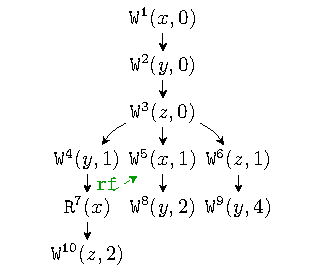
\includegraphics[scale=1]{figure/cuts/cut.pdf}
	\caption{The execution graph to be cut}
	\label{cut:to-be-cut}
\end{figure}
\michalis{rf is usually drawn from writes to reads.}

For revisit cut, since the read event has the greater stamp, the graph will be simply cut up until stamp = 7, shown in Figure~\ref{cut:revisit}.

\begin{figure}[htbp]
	\centering
	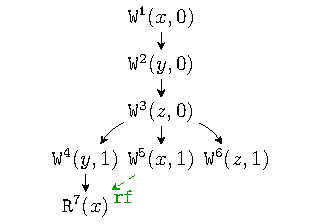
\includegraphics[scale=1]{figure/cuts/cut-revisit.pdf}
	\caption{Revisit cut output}
	\label{cut:revisit}
\end{figure}

For minimal cut, the fuzzer counts the porf predecessors of $\text{R}^7(x)$ and $\text{W}^5(x, 1)$. The events in the third thread (the rightmost column) will be removed. $\text{W}^{10}(z, 2)$ and $\text{W}^{8}(y, 2)$ are removed since they porf successors of porf successors of $\text{R}^7(x)$ and $\text{W}^5(x, 1)$, respectively. The resulting graph is shown in Figure~{cut:minimal}.

\begin{figure}[htbp]
	\centering
	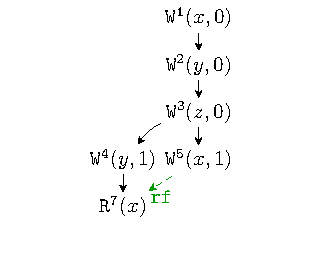
\includegraphics[scale=1]{figure/cuts/cut-minimal.pdf}
	\caption{Minimal cut output}
	\label{cut:minimal}
\end{figure}

For maximal cut, only the porf successors of the read, $\text{R}^7(x)$, will be removed. In this graph, $\text{W}^{10}(z, 2)$ will be removed with all other events remained, shown in Figure~\ref{cut:maximal}.

\begin{figure}[htbp]
	\centering
	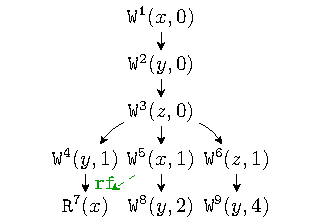
\includegraphics[scale=1]{figure/cuts/cut-maximal.pdf}
	\caption{Maximal cut output}
	\label{cut:maximal}
\end{figure}


\subsection{The is\_interesting function}



The \texttt{is\_interesting} function is defined as follows: we first compute the relative frequency for a graph:
\[
f_{\text{rel}}(g) = \frac{f_g^2}{\sum_{g_i \in G} {g_i}^2 / |G| },
\]
where \( f_{g_i} \) is the frequency of occurrences of the execution graph \( g_i \) in the set of explored graphs \( G \). For example, if the fuzzer explores graphs \( g_1 \), \( g_2 \), and \( g_3 \) 2, 3, and 5 times respectively in 10 total explorations, the relative frequency of \( g_1 \) is:
\[
\frac{2^2}{\left(2^2 + 3^2 + 5^2\right) / 3} \approx 0.32,
\]
and for \( g_3 \), it is:
\[
\frac{5^2}{\left(2^2 + 3^2 + 5^2\right) / 3} \approx 1.97.
\]
If the relative frequency is below a certain threshold, the corresponding execution graph is considered "interesting." For example, with a threshold of 0.4, \( g_1 \) is considered interesting, while \( g_3 \) is not.

This computation provides more granularity than simply checking if a graph is new. If we only flagged a graph as interesting when it's new, it could only be considered interesting once. By using frequencies, we refine this process. However, just using frequency is not always sufficient. For example, with a threshold of 0.2 in the above case, none of the graphs would be considered interesting, even though \( g_1 \) has a lower frequency than the others. In this case, the threshold of 0.2 is too low. In another scenario, if the fuzzer discovers 100 different graphs with frequencies like 0.01, 0.02, 0.015, etc., all lower than 0.1, they would all be considered interesting. But it would be reasonable to only prioritize those with relatively lower frequencies. In other words, the threshold is too high in this case. To address these issues, we use the relative frequency, which takes into account both the graph's frequency and those of others. Squaring the frequencies amplifies differences and avoids discarding the sum, which is always 1.


% \frac{f_g}{\sum_{g_i \in G} f_{g_i}^2 / N_G}

\section{Benchmarks}

We use the following benchmarks to evaluate the fuzzer.

% \paragraph{big0} A syntactic benchmark with multiple threads reading from and writing to shared memory locations using acquire-release memory orders.

\paragraph{ring-buffer} A ring buffer implementation in FreeBSD 8.0.0. Each thread enqueues a message and dequeues one from the buffer. The program checks the correctness and integrity of the messages. The ring buffer uses an array to store data. The enqueue and dequeue operations use compare-and-swap loops to update the queue head and tail pointers.

% \paragraph{fib} Two threads update a Fibonacci sequence concurrently. Each update uses the previous values of two variables.

\paragraph{mpmc-queue} A multi-producer multi-consumer bounded queue implementation. It maintains three state variables that keeps track of the number of reads and writes that have been started and finished. Each writer obtains an index in the queue's array buffer using cas loop and write to that position. The readers will increment the reading index and read the data. In the test, 2 readers and 4 writers are spawned.

% \paragraph{szymanski} A szymanski mutual exclusion algorithm implementation. Each thread has a flag to inidicate its state. Before entering critical section, each thread updates its own flag and checks the other thread's flag. SC atomic fences are used for synchronization.


\paragraph{ttaslock} A spinlock called Test-and-Test-and-Set (TTAS) lock. The lock has an atomic state variable shared by multiple threads. Before locking it, a thread first loads the flag and wait until it is not set. Locking is implemented using a loop that exchanges the state value until the old value of it is not set. In the benchmark, two threads are luanched to update a non-atomic shared variable and asserts they read their values in the critical section.

\paragraph{treiber-stack} A treiber stack\cite{treiber-stack} implementation using compare-and-swap for pushing and popping nodes.

\paragraph{ms-queue} An ms-queue implementation similar to that in the previous chapter, written in C.

\paragraph{linuxrwlocks} The reader-writer lock implementation of linux kernel, similar to that in the previous chapter but written in C.

\paragraph{long-assert} A test case that has a complicated assertion that is hard to trigger. One thread checks the assertion involving two shared variables and the other thread modifies one of them after doing some exponential work.

\section{Evaluation and discussion}

\paragraph*{Research questions} Below lists the research questions we want to explore.

\begin{enumerate}[label=RQ\arabic*,resume]
	\item Is the fuzzer able to explore more distinct execution graphs in a fixed number of iterations than the random tester? \label{RQ:CutVSRandom}
	\item Among the three mutation strategies, which performs best? Why? \label{RQ:CutComparison}
	\item What's the runtime performance of the fuzzer with different mutations, comparing with random testing? \label{RQ:GenMCOverhead}
	\item Is the fuzzer able to find bugs faster than the model checker?\label{RQ:GenMC_vs_fuzzer}
\end{enumerate}

\subsection{\ref*{RQ:CutVSRandom}: Fuzzer vs random tester }

To address this question, we run both the fuzzer and the GenMC in its estimation mode for 10 thousand iterations. Using the hash function defined in section~\ref{sec:hashf}, we count the number of distinct execution graphs they found. Table~\ref{genmc:num-of-exe} shows the results of each benchmark. The improvements are computed by:
\[
	R_{improvement} = \frac{\frac{1}{3} (N_{revisit}+N_{minimal}+N_{maximal}) - N_{random} }{N_{random}} \times 100 \%.
\]

\begin{table}[h!]
	\centering
	\begin{tabular}{|c|cccc|c|}
		\hline
		\diagbox{Benchmark}{ Strategy} & random & revisit cut & minimal cut & maximal cut & $R_{improvement}$ \\ \hline
		ring-buffer                    & 6953   & 16449       & 30803       & 49290       & 362.83\%          \\ \hline
		linuxrwlocks                   & 9658   & 10699       & 27459       & 20666       & 103.02\%          \\ \hline
		mpmc-queue                     & 23145  & 49506       & 53003       & 66422       & 143.29\%          \\ \hline
		ms-queue                       & 13746  & 31404       & 23078       & 32792       & 111.63\%          \\ \hline
		treiber-stack                  & 9029   & 28005       & 41201       & 53892       & 354.45\%          \\ \hline
		ttaslock                       & 8633   & 8982        & 10430       & 10245       & 14.51\%           \\ \hline
	\end{tabular}
	\label{genmc:num-of-exe}
	\caption{Number of unique execution graphs of each exploration strategy}
\end{table}

It can be observed that for all of the above benchmarks, the fuzzer is able to explore higher number of execution graphs than the random tester does. The average improvement, computed by


\[
	\overline{R_{\text{improvement}}} = \frac{1}{n} \sum N_{improvement}
\]
is 181.62\%.

\subsection{\ref*{RQ:CutComparison}: Revisit cut vs minimal cut vs maximal cut }

Figure~\ref{genmc:buf_ring} to \ref{genmc:ttaslock} show the execution graph coverage plots of random testing and fuzzing with three mutation strategies. It can be seen that in 5 of these benchmarks, the maximal cut finds the greatest number of execution graphs. The revisit cut performs the best in 2 benchmarks.

\begin{figure}[h!]

	\centering
	\begin{minipage}{0.45\textwidth}
		\centering
		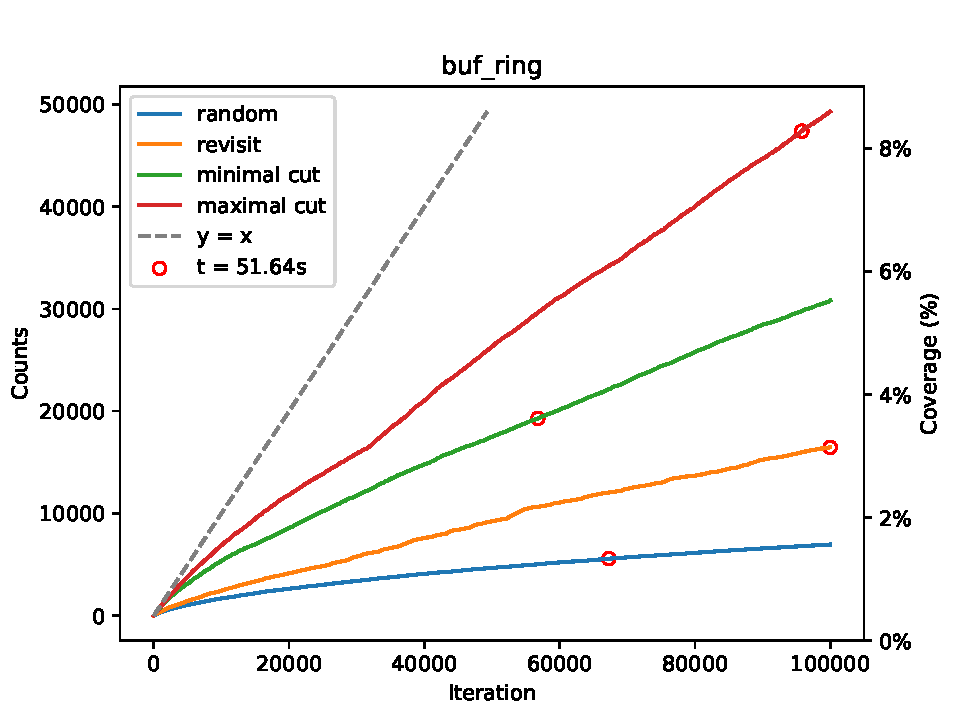
\includegraphics[width=\textwidth]{figure/genmc/buf_ring.pdf}
		\caption{ring-buffer (search space size: 547177)}
		\label{genmc:buf_ring}
	\end{minipage}
	\hfill
	\begin{minipage}{0.45\textwidth}
		\centering
		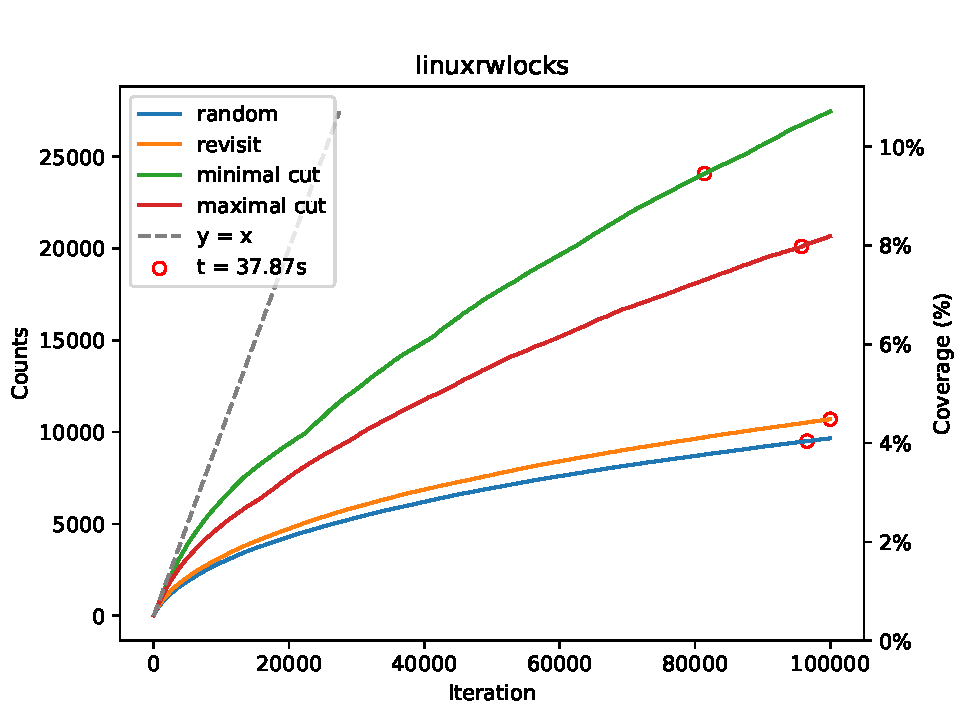
\includegraphics[width=\textwidth]{figure/genmc/linuxrwlocks.pdf}
		\caption{linuxrwlocks (search space size: 244756)}
		\label{genmc:linuxrwlocks}
	\end{minipage}

	\vspace{0.5cm}

	\begin{minipage}{0.45\textwidth}
		\centering
		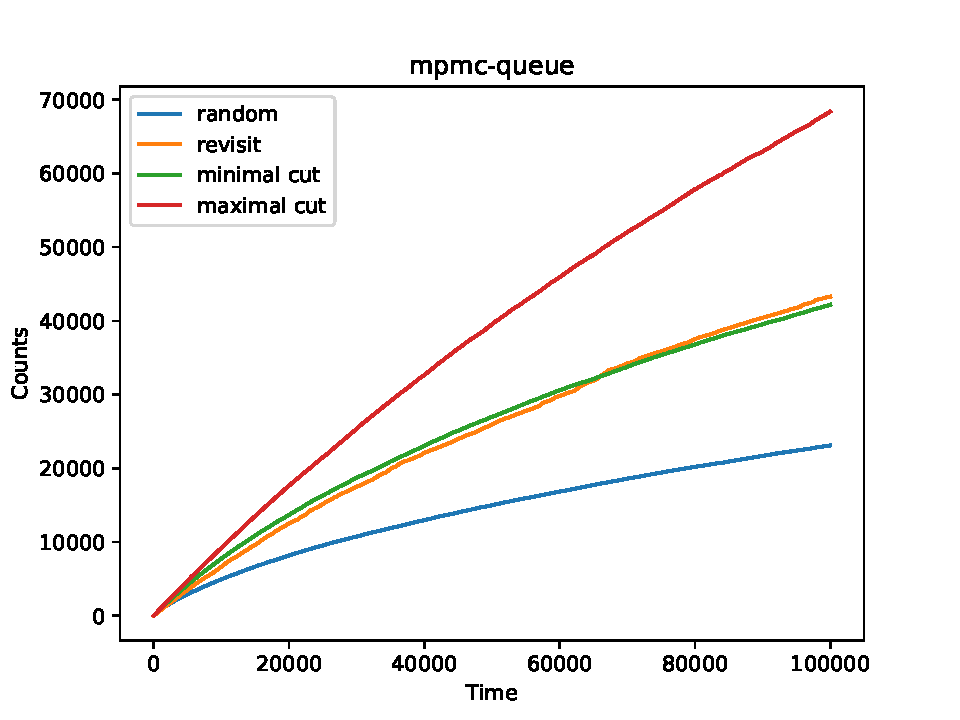
\includegraphics[width=\textwidth]{figure/genmc/mpmc-queue.pdf}
		\caption{mpmc-queue (search space size: 417468)}
		\label{genmc:mpmc-queue}
	\end{minipage}
	\hfill
	\begin{minipage}{0.45\textwidth}
		\centering
		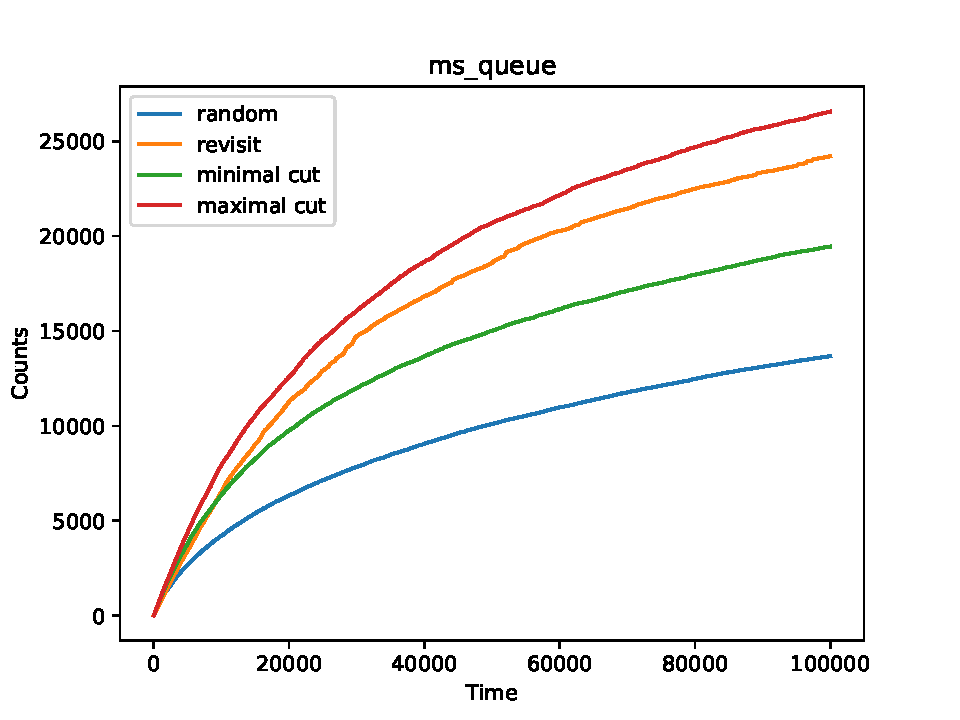
\includegraphics[width=\textwidth]{figure/genmc/ms_queue.pdf}
		\caption{ms-queue (search space size: 97604)}
		\label{genmc:ms-queue}
	\end{minipage}

	\vspace{0.5cm}

	\begin{minipage}{0.45\textwidth}
		\centering
		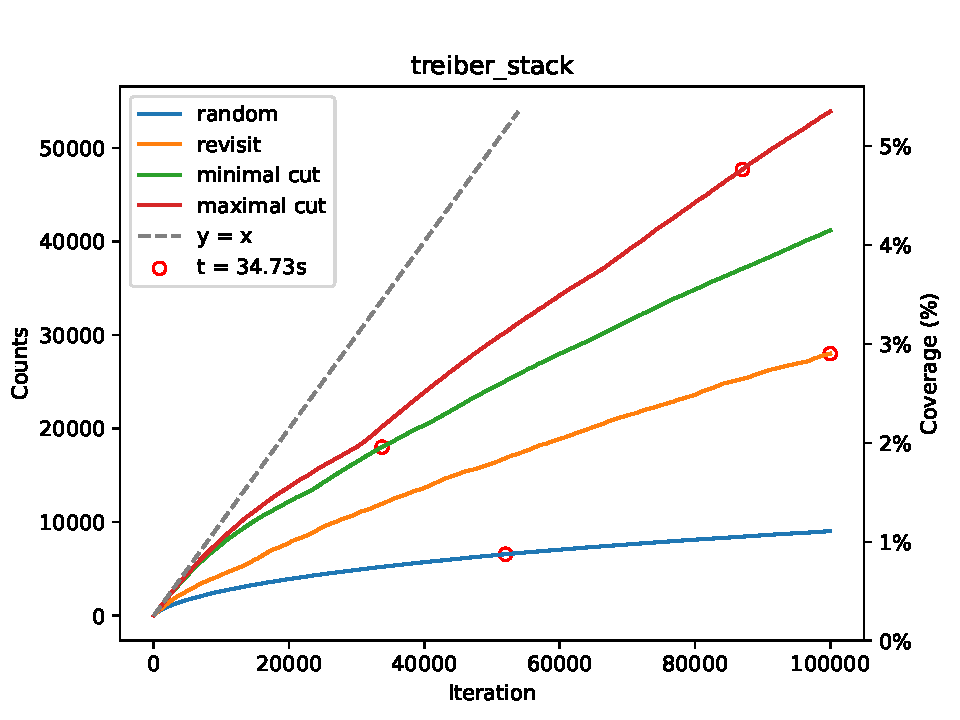
\includegraphics[width=\textwidth]{figure/genmc/treiber_stack.pdf}
		\caption{treiber-stack (search space size: 961851)}
		\label{genmc:treiber_stack}
	\end{minipage}
	\hfill
	\begin{minipage}{0.45\textwidth}
		\centering
		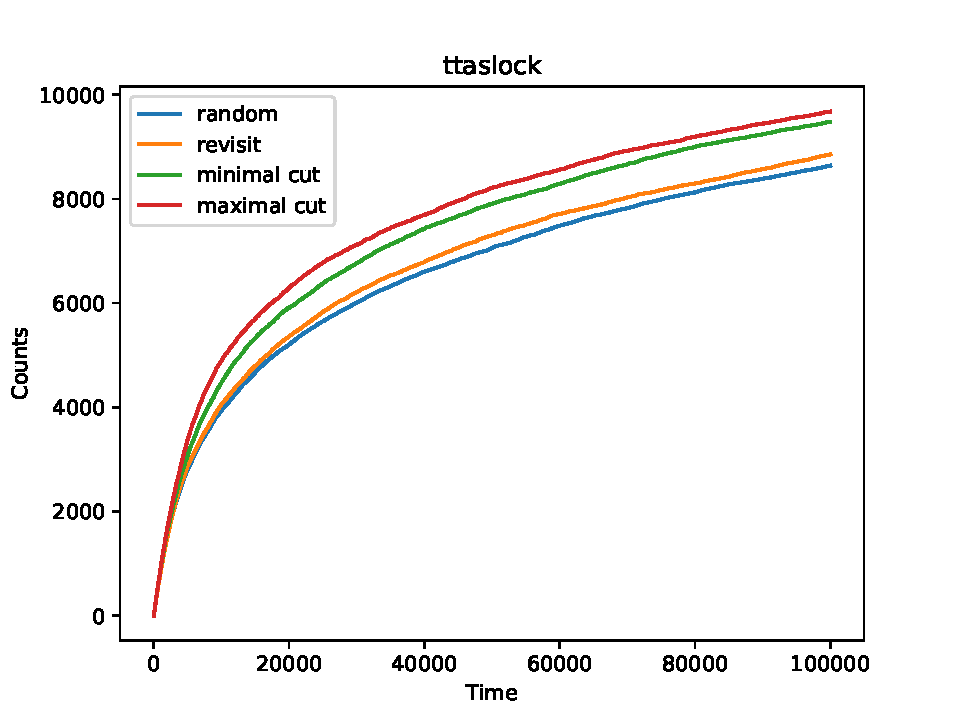
\includegraphics[width=\textwidth]{figure/genmc/ttaslock.pdf}
		\caption{ttaslock (search space size: 49678)}
		\label{genmc:ttaslock}
	\end{minipage}

	% \vspace{0.5cm}
	% \begin{minipage}{0.45\textwidth}
	% 	\centering
	% 	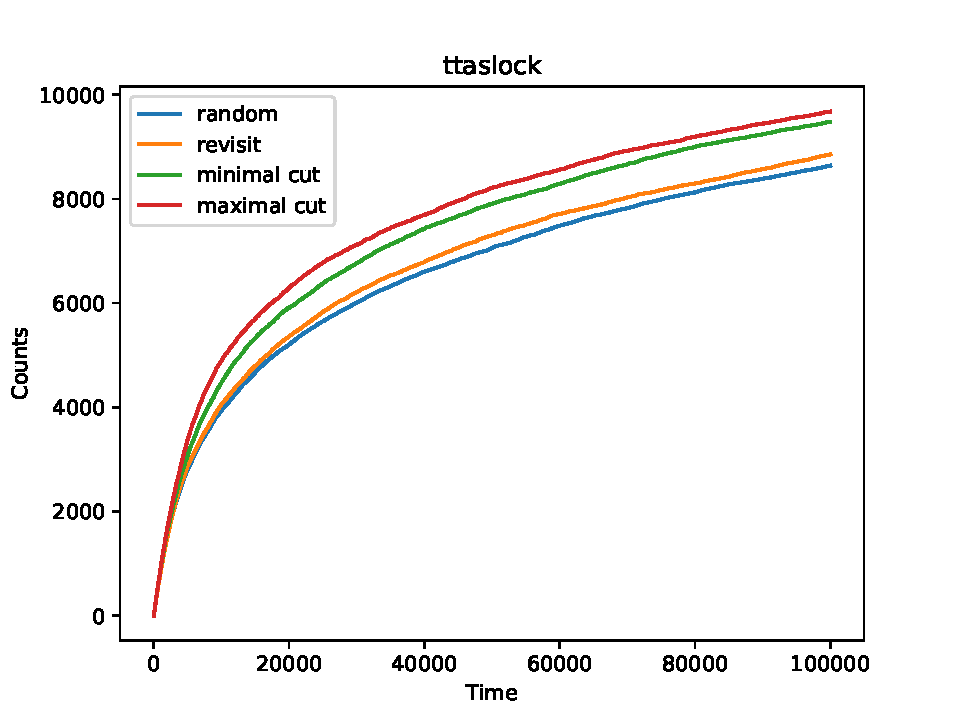
\includegraphics[width=\textwidth]{figure/genmc/ttaslock.pdf}
	% 	\caption{ttaslock}
	% 	\label{genmc:ttaslock}
	% \end{minipage}
	% \hfill
	% \begin{minipage}{0.45\textwidth}
	% 	\centering
	% 	% This empty minipage will help the last image to be aligned to the left
	% \end{minipage}
\end{figure}




It is hypothesized that the performance is related to the number of events that remain in the mutated graph. Generally, the more events that are preserved in the mutated graph, the closer their relations tend to be. The random strategy, for example, can be seen as a method that cuts out the whole portion of the graph, resulting in the fewest remaining events. To better understand this relationship, we measured the average number of events in execution graphs for each benchmark, as well as the average number of events that remain after applying each cutting strategy, as shown in Table~\ref{genmc:average-events}. The data shows that, in the benchmarks linuxrwlocks and ttaslock, the revisit cut strategy retains the highest number of events in their mutated graphs and performs best in discovering more execution graphs. Similarly, in other benchmarks, the maximal cut strategy retains the highest number of events and explores the largest number of distinct graphs. Overall, the results indicate that the number of explored execution graphs is positively correlated with the number of events remaining in the mutation strategies.



\begin{table}[h!]
	\centering
	\begin{tabular}{|c|cccc|}
		\hline
		\diagbox{Benchmark}{ Strategy} & total  & revisit cut & minimal cut & maximal cut \\ \hline
		ring-buffer                    & 102.18 & 81.88       & 41.15       & 94.11       \\ \hline
		linuxrwlocks                   & 77.26  & 59.79       & 30.79       & 54.03       \\ \hline
		mpmc-queue                     & 85.24  & 59.57       & 31.75       & 73.95       \\ \hline
		ms-queue                       & 172.85 & 136.00      & 66.13       & 159.68      \\ \hline
		treiber-stack                  & 113.50 & 83.98       & 53.51       & 99.49       \\ \hline
		ttaslock                       & 65.35  & 59.41       & 21.76       & 51.88       \\ \hline
	\end{tabular}
	\label{genmc:average-events}
	\caption{Number of events in original graphs and mutated graphs, on average}
\end{table}





\subsection{\ref*{RQ:GenMCOverhead}: Runtime overhead and efficiency of 3 mutations }

We examine the total time elapsed for exploring 100 thousand iterations, shown in Figure~\ref{genmc:overhead}. The random testing is taken as a baseline for evaluating the overhead. It can be seen that random testing does not always take the shortest time. This is due to the mechanism of GenMC. When adding events to the graph, the GenMC driver first inspects whether there is already an event in that position. If so, it continues without the need to check consistency, pick rf's, or arrange it in the coherence order. Although the maximal cut takes many steps to compute the cut view, it still takes the shortest time in one of the benchmarks since the driver can save effort on those remaining events. Overall, all three mutations have insignificant effects on the runtime performance, with affordable overheads.




\begin{figure}[h!tbp]
	\centering
	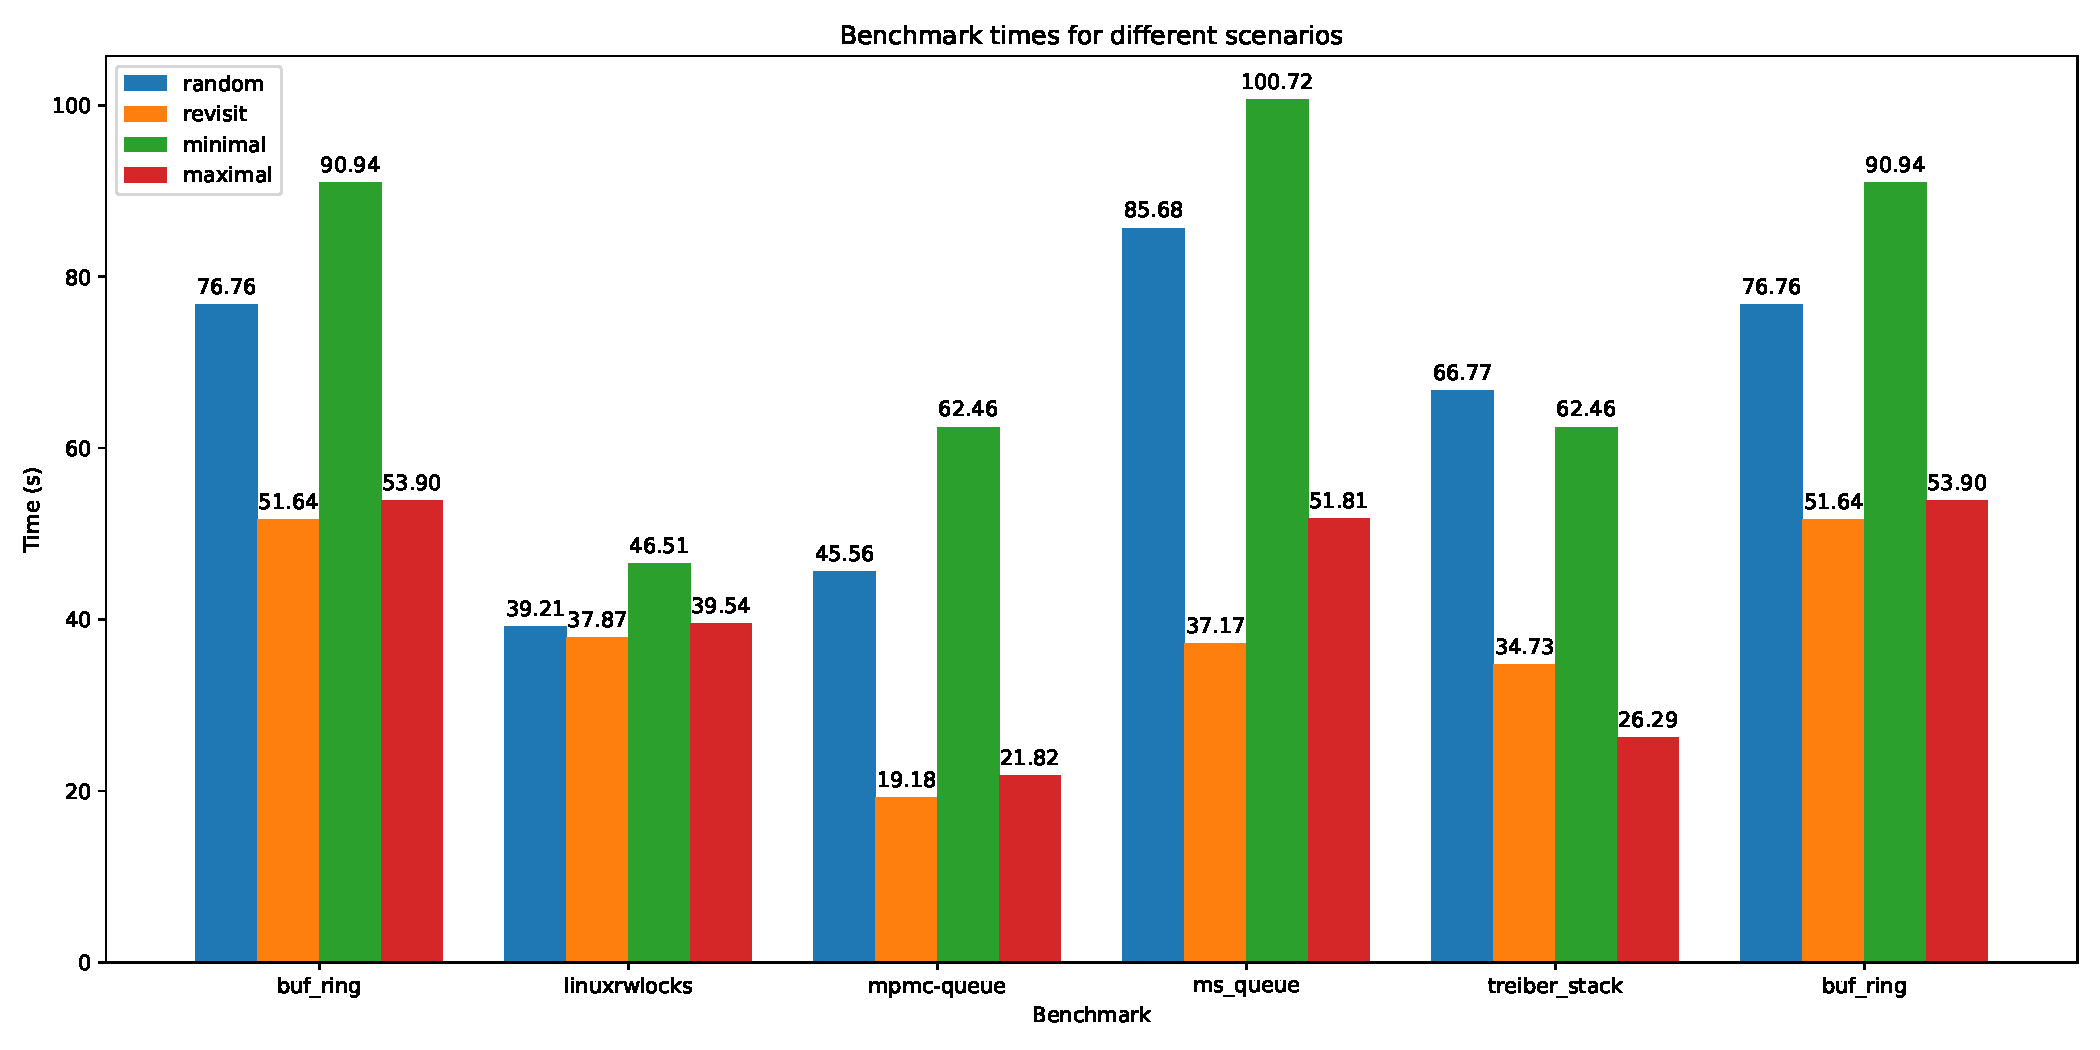
\includegraphics[scale=0.37]{figure/genmc/overhead.pdf}
	\caption{Time elapsed by various strategies}
	\label{genmc:overhead}
\end{figure}

In addition, it is possible that one strategy may find more execution graphs in a fixed number of iterations than another but takes more time to complete. Therefore another concern is the efficiency of various mutations, defined as $\sigma_T = \frac{N_{graph}}{T}$, where $N_{graph}$ is the number of distinct execution graphs, and $t$ is a fixed time. Note that this ratio is not a constant value over time, as it becomes increasingly difficult to explore new execution graphs as time progresses. Here we set $T$ to be 1 minute and count the number of different execution graphs explored. The results are shown in Figure~\ref{genmc:buf_ring-time} to Figure~\ref{genmc:ttaslock-time}. Our results indicate that the maximal cut has the highest efficiency in a majority of benchmarks, while the random tester generally has the lowest efficiency.



\begin{figure}[h!]

	\centering
	\begin{minipage}{0.45\textwidth}
		\centering
		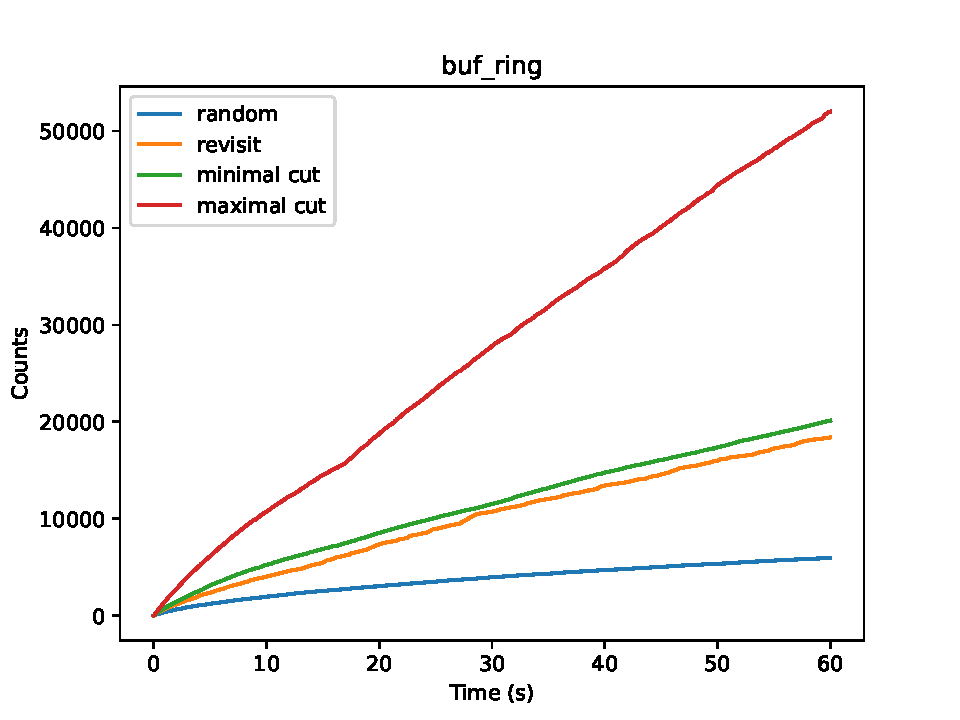
\includegraphics[width=\textwidth]{figure/genmc-time/buf_ring.pdf}
		\caption{ring-buffer}
		\label{genmc:buf_ring-time}
	\end{minipage}
	\hfill
	\begin{minipage}{0.45\textwidth}
		\centering
		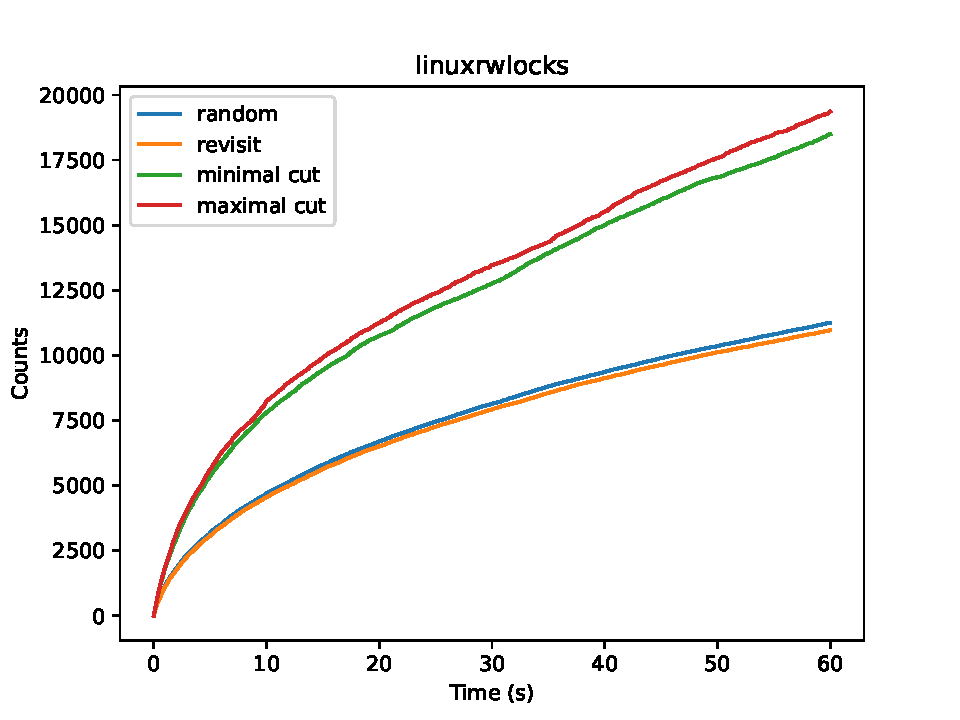
\includegraphics[width=\textwidth]{figure/genmc-time/linuxrwlocks.pdf}
		\caption{linuxrwlocks}
		\label{genmc:linuxrwlocks-time}
	\end{minipage}

	\vspace{0.5cm}

	\begin{minipage}{0.45\textwidth}
		\centering
		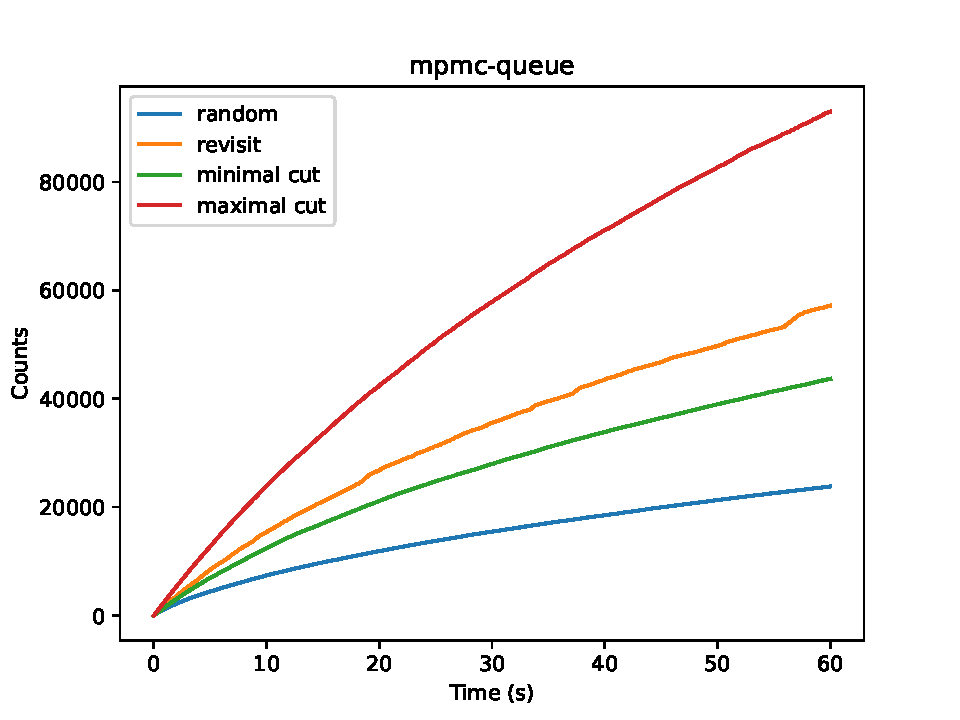
\includegraphics[width=\textwidth]{figure/genmc-time/mpmc-queue.pdf}
		\caption{mpmc-queue}
		\label{genmc:mpmc-queue-time}
	\end{minipage}
	\hfill
	\begin{minipage}{0.45\textwidth}
		\centering
		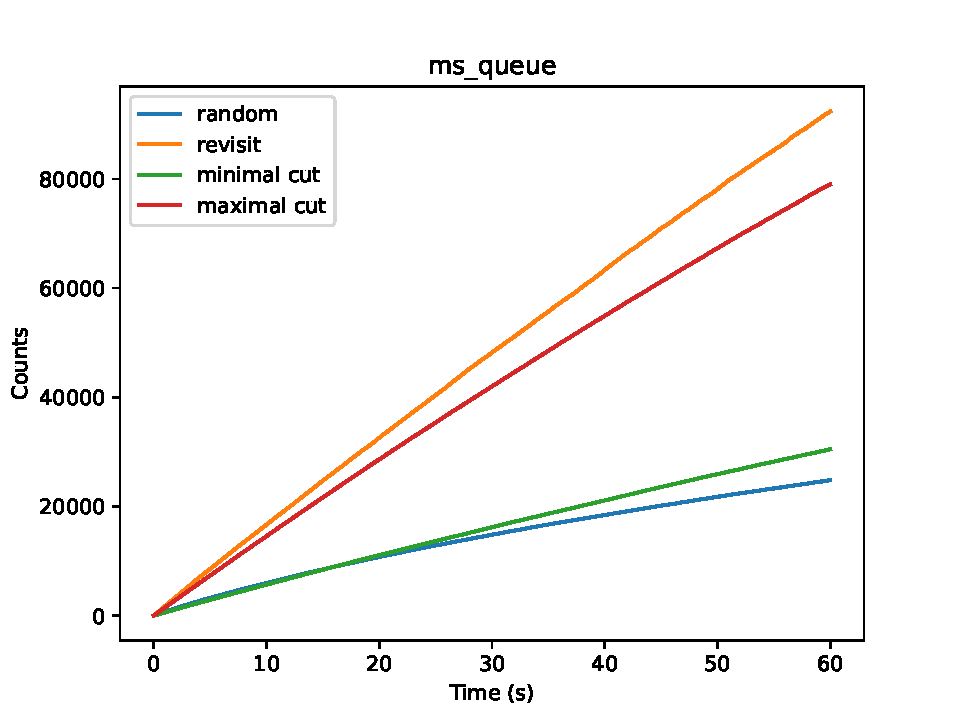
\includegraphics[width=\textwidth]{figure/genmc-time/ms_queue.pdf}
		\caption{ms-queue}
		\label{genmc:ms-queue-time}
	\end{minipage}

	\vspace{0.5cm}

	\begin{minipage}{0.45\textwidth}
		\centering
		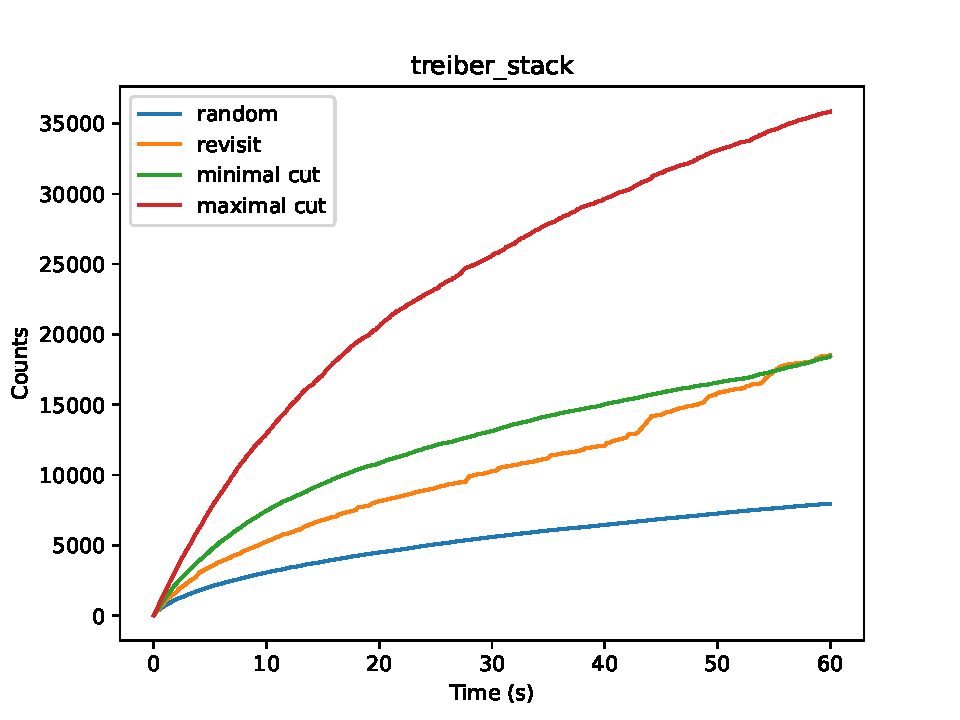
\includegraphics[width=\textwidth]{figure/genmc-time/treiber_stack.pdf}
		\caption{treiber-stack}
		\label{genmc:treiber_stack-time}
	\end{minipage}
	\hfill
	\begin{minipage}{0.45\textwidth}
		\centering
		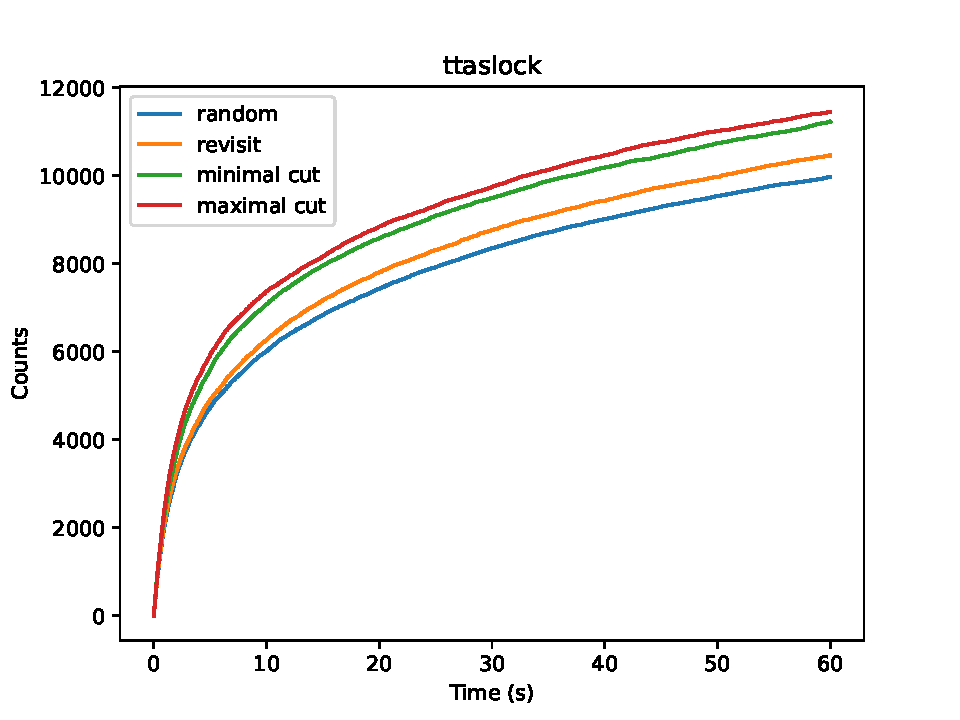
\includegraphics[width=\textwidth]{figure/genmc-time/ttaslock.pdf}
		\caption{ttaslock}
		\label{genmc:ttaslock-time}
	\end{minipage}
\end{figure}



\subsection{\ref*{RQ:GenMC_vs_fuzzer}: Fuzzer vs model checker }

Model checkers are also used to verify the correctness of programs and detect bugs. The GenMC model checker implements an optimal algorithm that ensures no duplication while enumerating execution graphs. However, we would like to demonstrate that in some cases, introducing randomness can be more efficient in terms of the number of iterations taken and the time elapsed for detecting a bug. Take the long-assert benchmark for example, as shown in Listing~\ref{long-assert}. In order to violate the assertion, \texttt{x} should read from its initial value while \texttt{y} reads the values 1, 2, 3, 4, and 5, sequentially. In the GenMC's verification process of this program, when the read of \texttt{x} event is added, the driver picks a value for it and pushes other alternative choices to the workqueue, which will be revisited later. Suppose the driver picks a non-zero value, the zero value will be tried again only after the drivers finish exploring graphs with the non-zero choice.


\begin{lstlisting}[caption={long-assert}, label={long-assert}]
	atomic_int x, y;

	void* thread_0(void* ) {
		x = 42;
	}

	void* thread_1(void* ) {
		// fails when x==0, y==1, y==2, y==3, ...
		assert(x != 0 || y != 1 || y != 2 || y != 3 || y != 4 || y != 5);  
	}

	void* thread_n(void* unused) {
		atomic_fetch_add(&y, 1);
	}

	void* thread_2(void* unused) {
		pthread_t t[N];	// N is a hyper parameter
		for (int i = 0U; i < N; i++) {	// y++, ++, ++...
			pthread_create(&t[i], NULL, thread_n, NULL);
		}			
		for (int i = 0U; i < N; i++) {	// join threads
			pthread_join(t[i], NULL);
		}			
		// cas on x after exponential work on y
		atomic_fetch_add(&x, 1);
	}

	int main() {
		pthread_t t0, t1, t2;
		pthread_create(&t0, NULL, thread_0, NULL);
		pthread_create(&t1, NULL, thread_1, NULL);
		pthread_create(&t2, NULL, thread_2, NULL);
		// join threads...
	}

\end{lstlisting}

Comparing the model checker, the random tester, and the fuzzer with revisit, minimal and maximal cuts, Figure~\ref{long-assert-N5-iter} and Figure~\ref{long-assert-N5-time} show the average number of iterations (for the model checker, this is the number of graphs prior to the buggy one) and the time taken to find the bug, respectively, with \texttt{N} taken from 5 to 9. It can be observed that the random tester and the fuzzer require fewer iterations to find the bug in all cases. When \texttt{N} is small, the model checker is faster, but as \texttt{N} increases, the fuzzer and random tester become faster.

\begin{figure}[h!tbp]
	\centering
	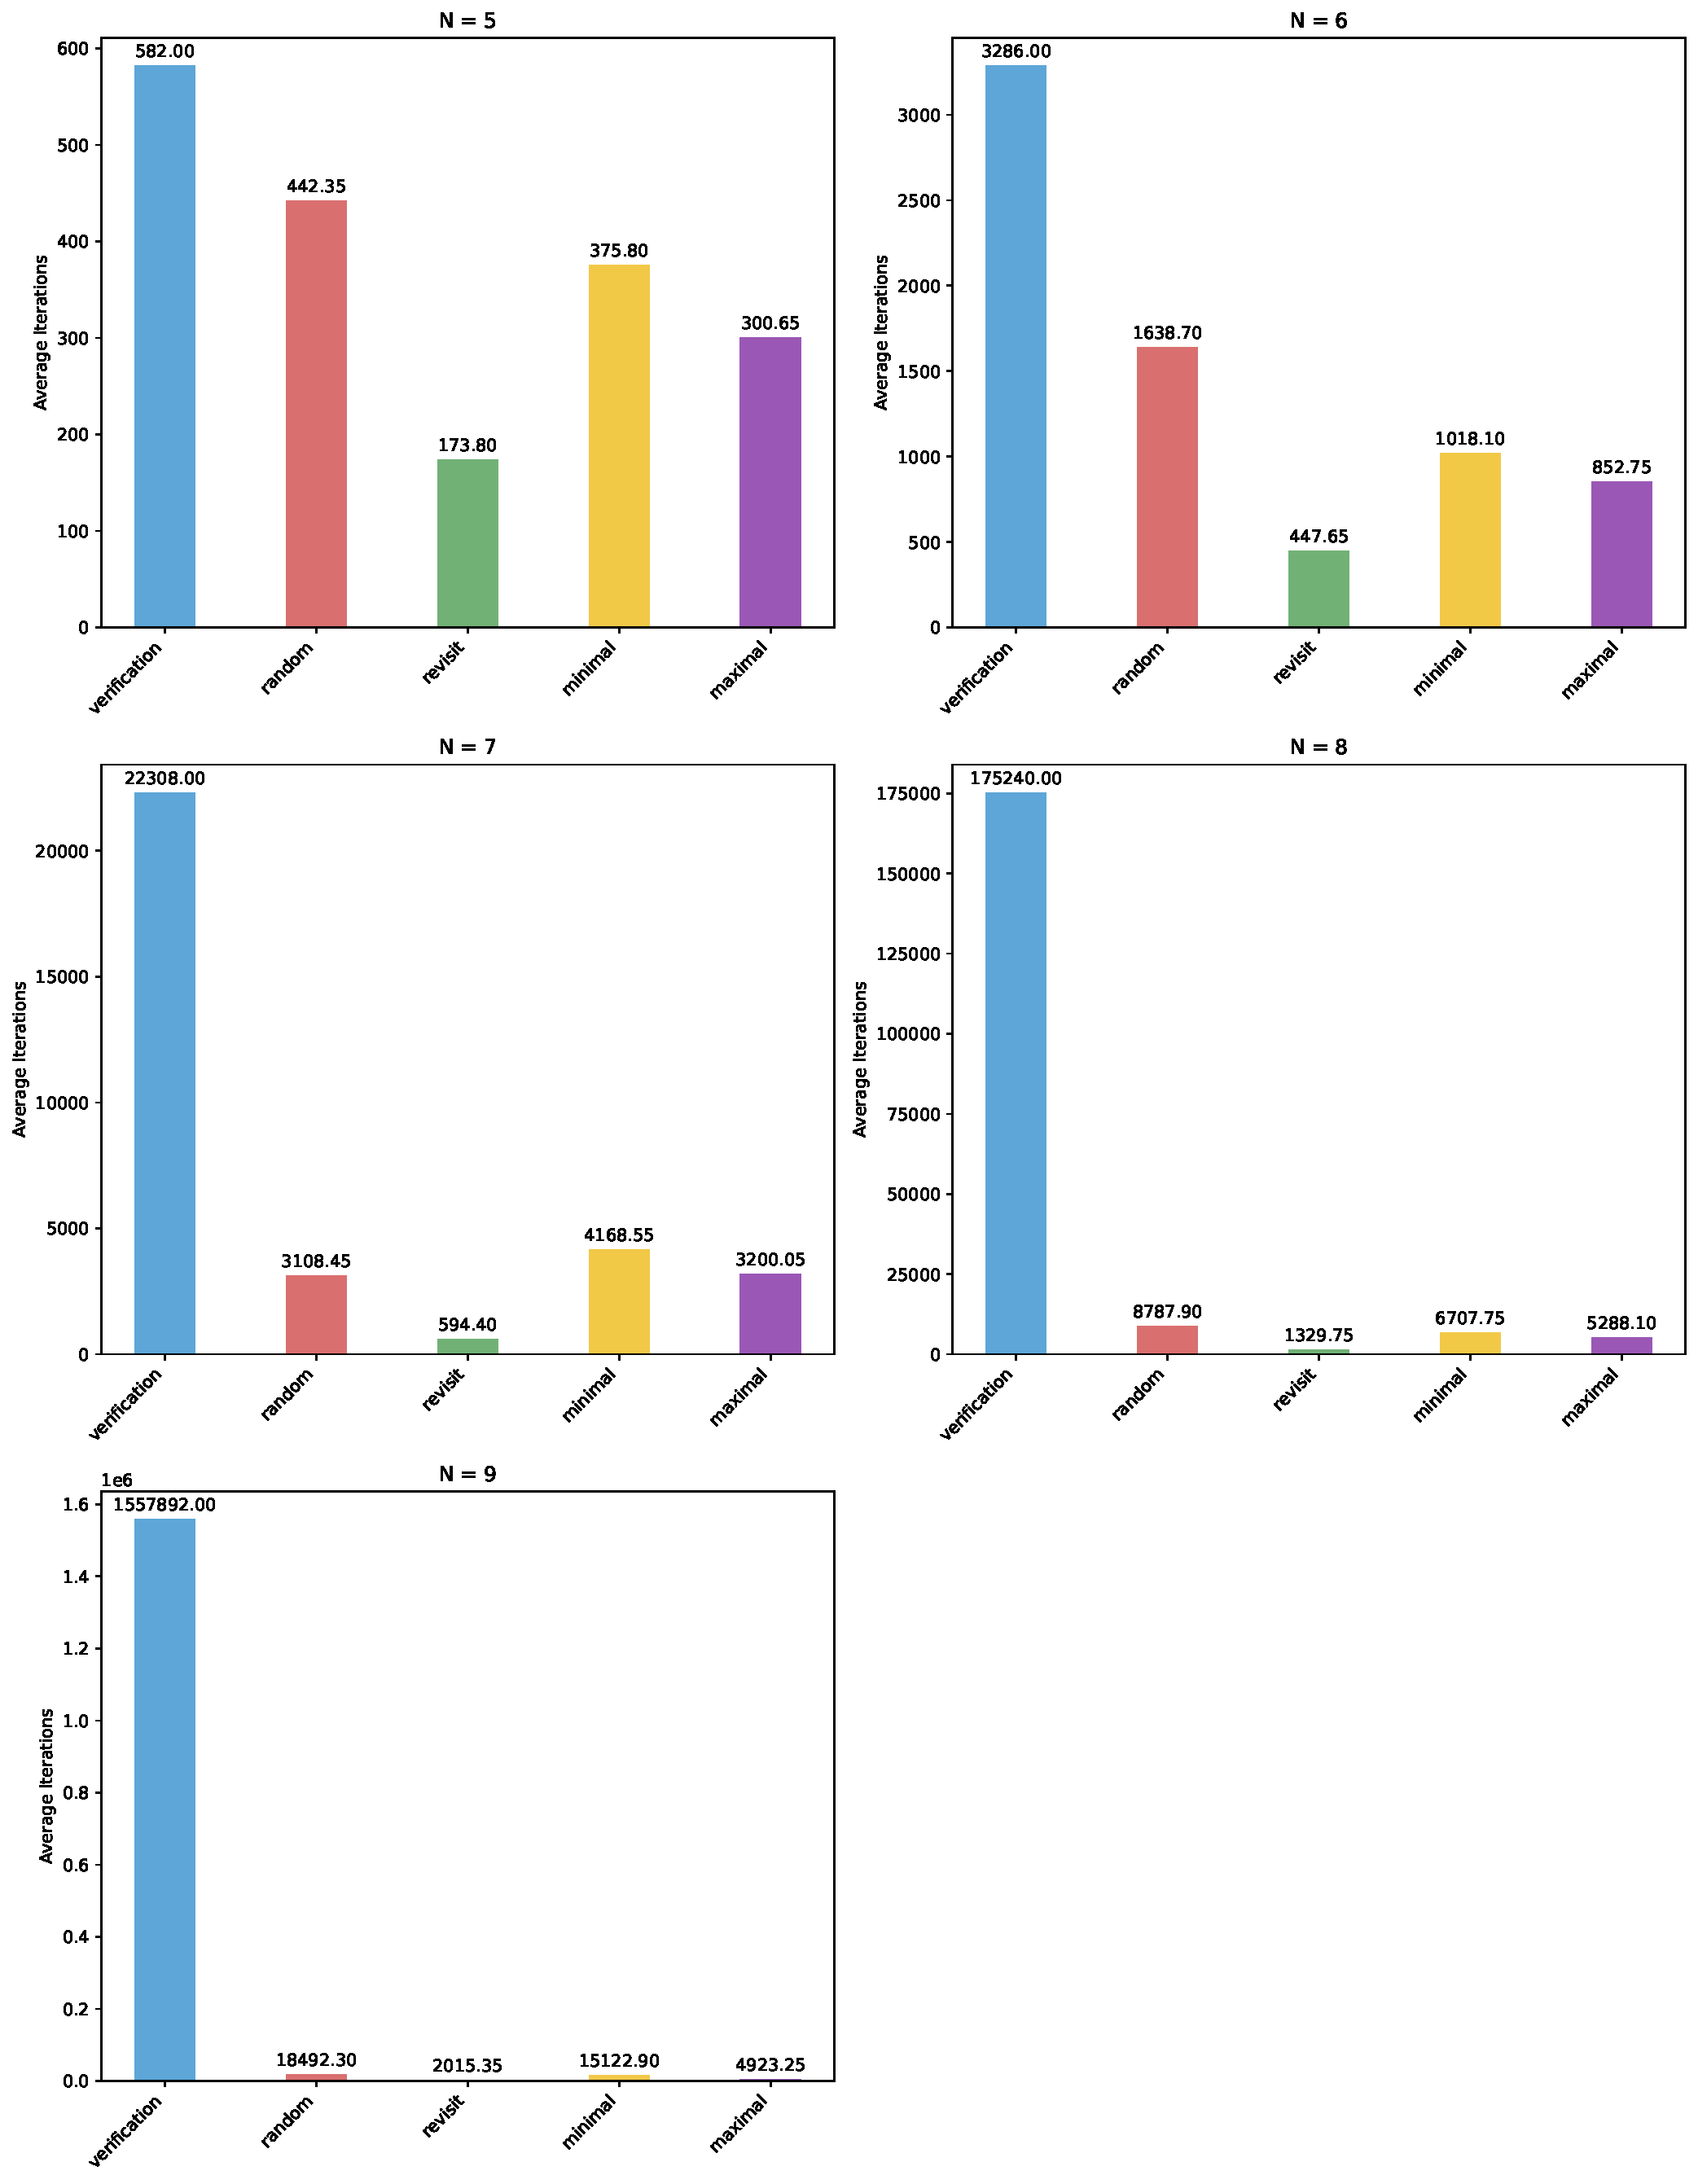
\includegraphics[scale=0.3]{figure/long-assert/fuzz_assert5_iter.pdf}
	\caption{Average iterations to detect the bug}
	\label{long-assert-N5-iter}
\end{figure}


\begin{figure}[h!tbp]
	\centering
	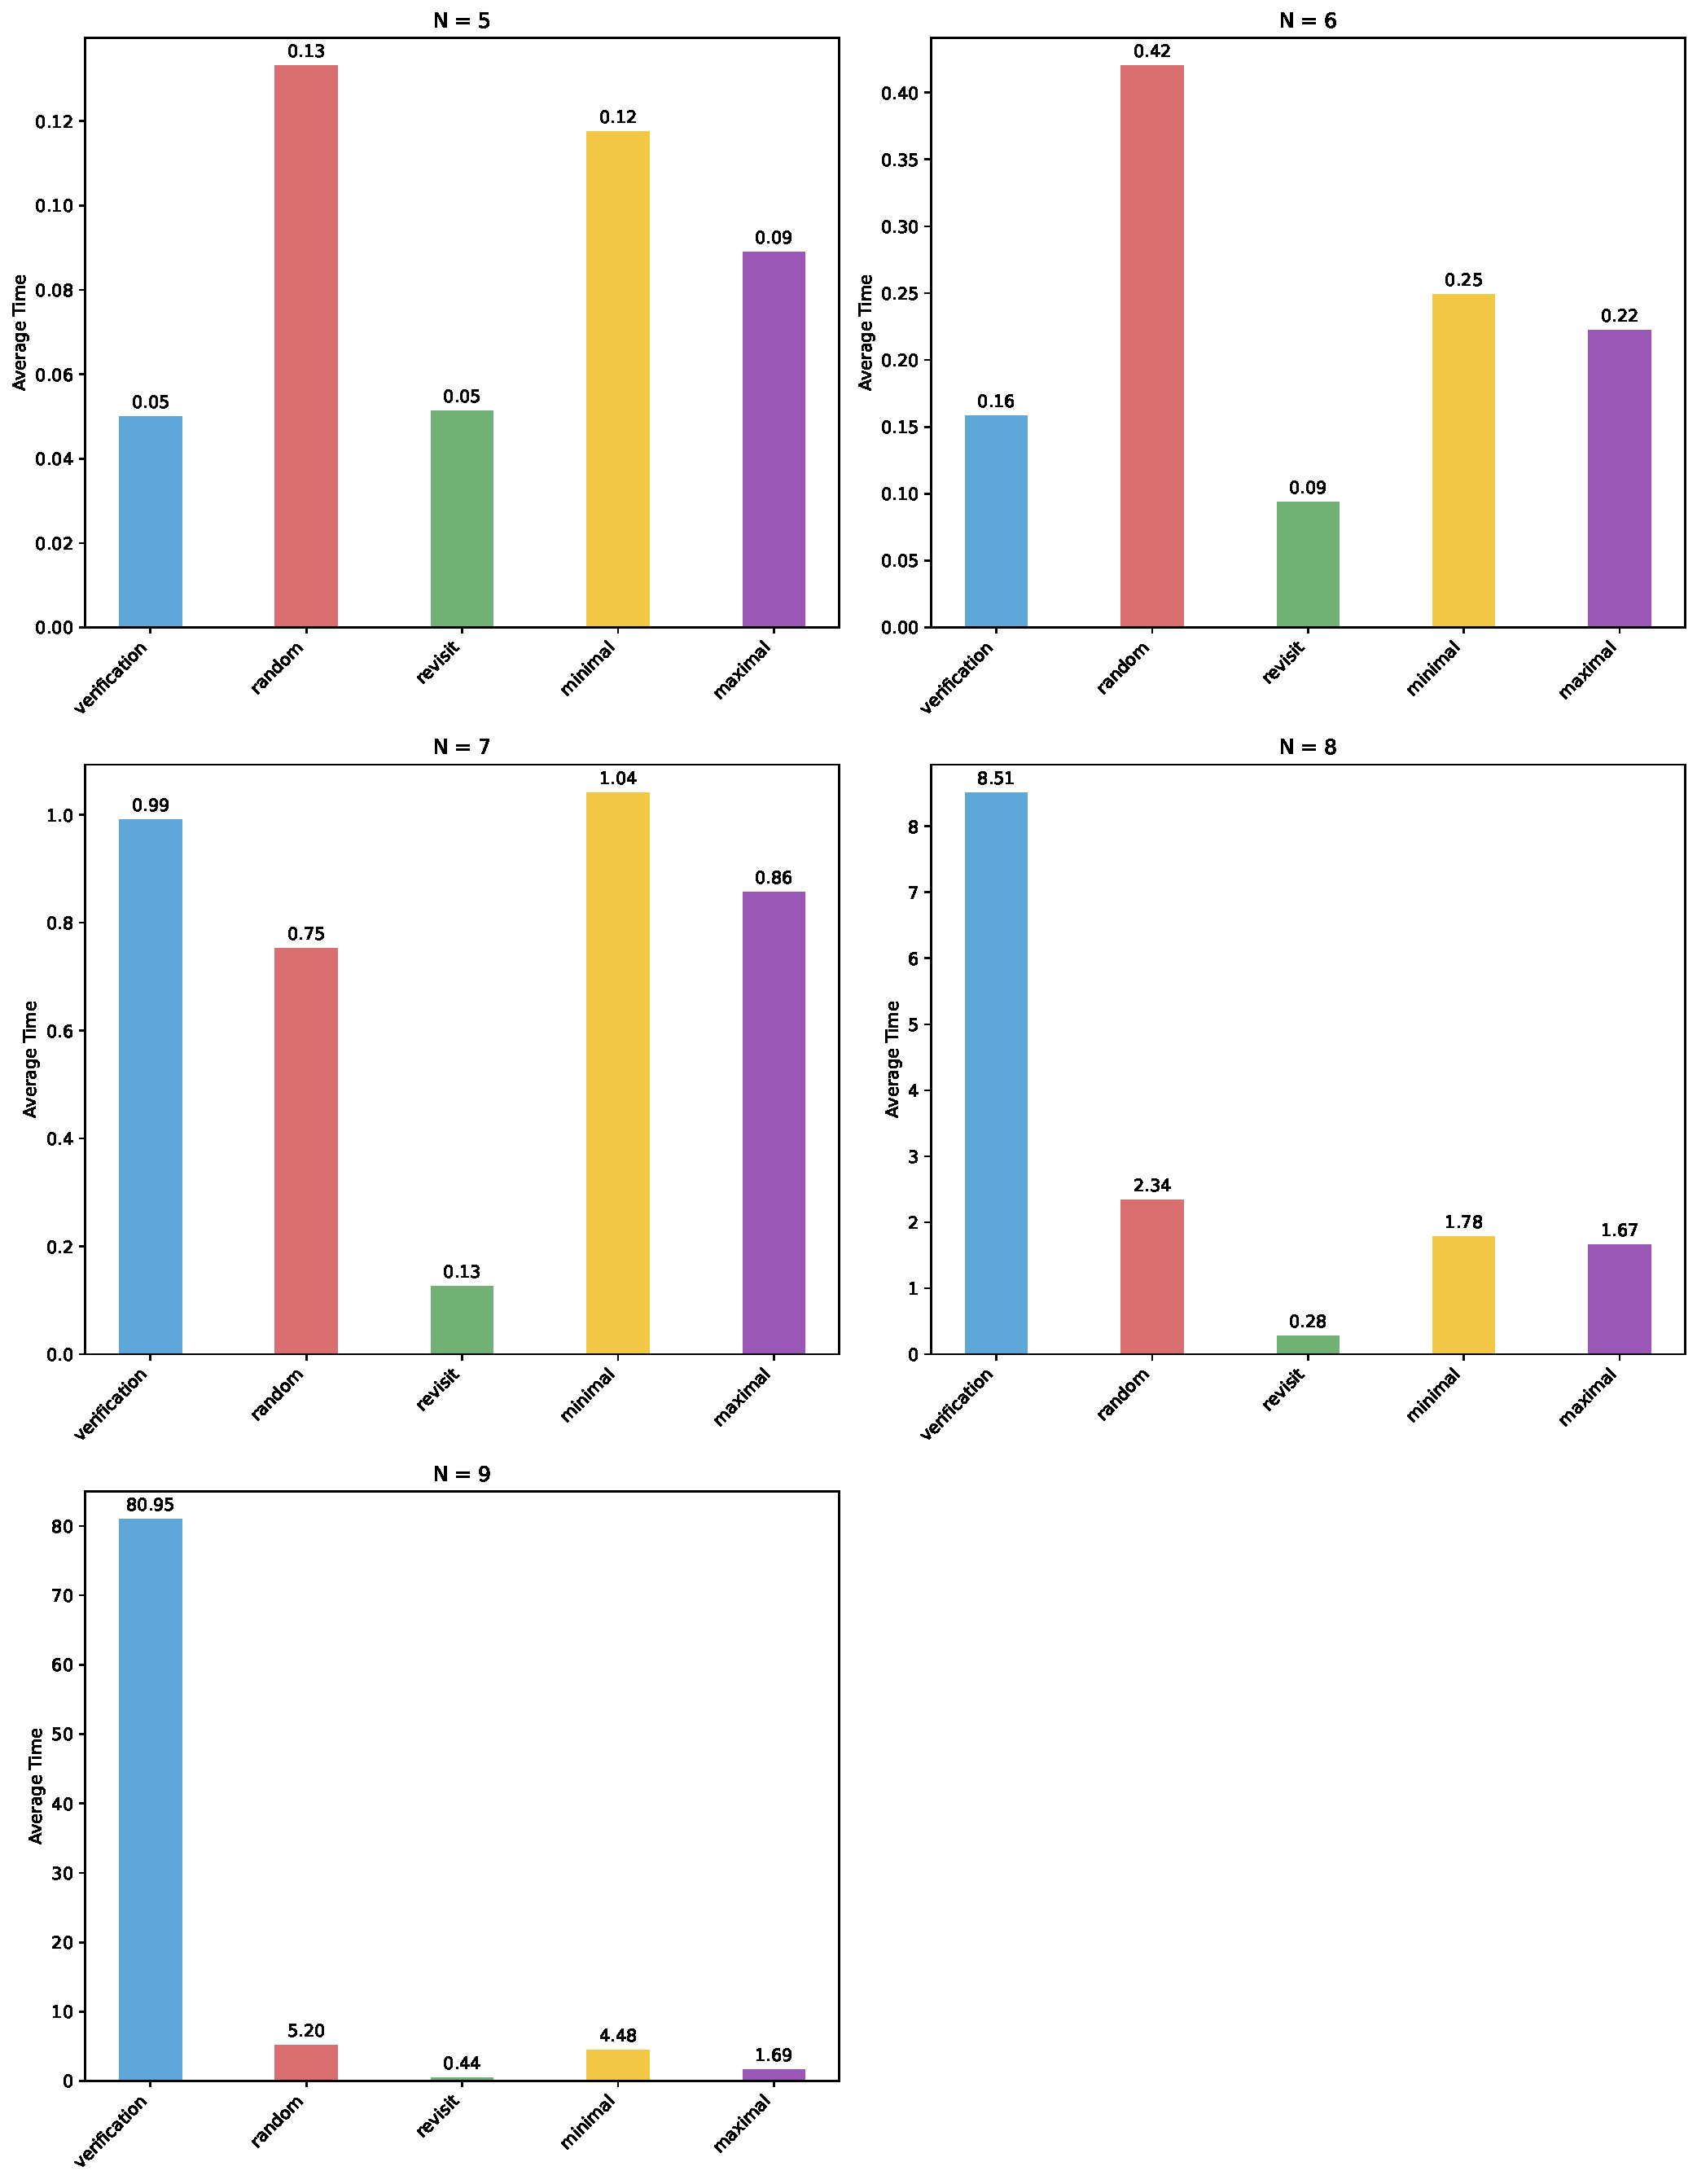
\includegraphics[scale=0.3]{figure/long-assert/fuzz_assert5_time.pdf}
	\caption{Average time to detect the bug}
	\label{long-assert-N5-time}
\end{figure}

If we change the assertion to \texttt{assert(x!=0||y!=1||y!=2||...||y!=N)}, it becomes increasingly difficult to find the bug as \texttt{N} gets larger. As shown in Figure~\ref{long-assert-N-time} and Figure~\ref{long-assert-N-iter}, the fuzzer with different mutations can take less time and iterations than the random tester. The model checker is not the most time consuming strategy this time but still the revisit cut can take less time to find the bug.


\begin{figure}[h!tbp]
	\centering
	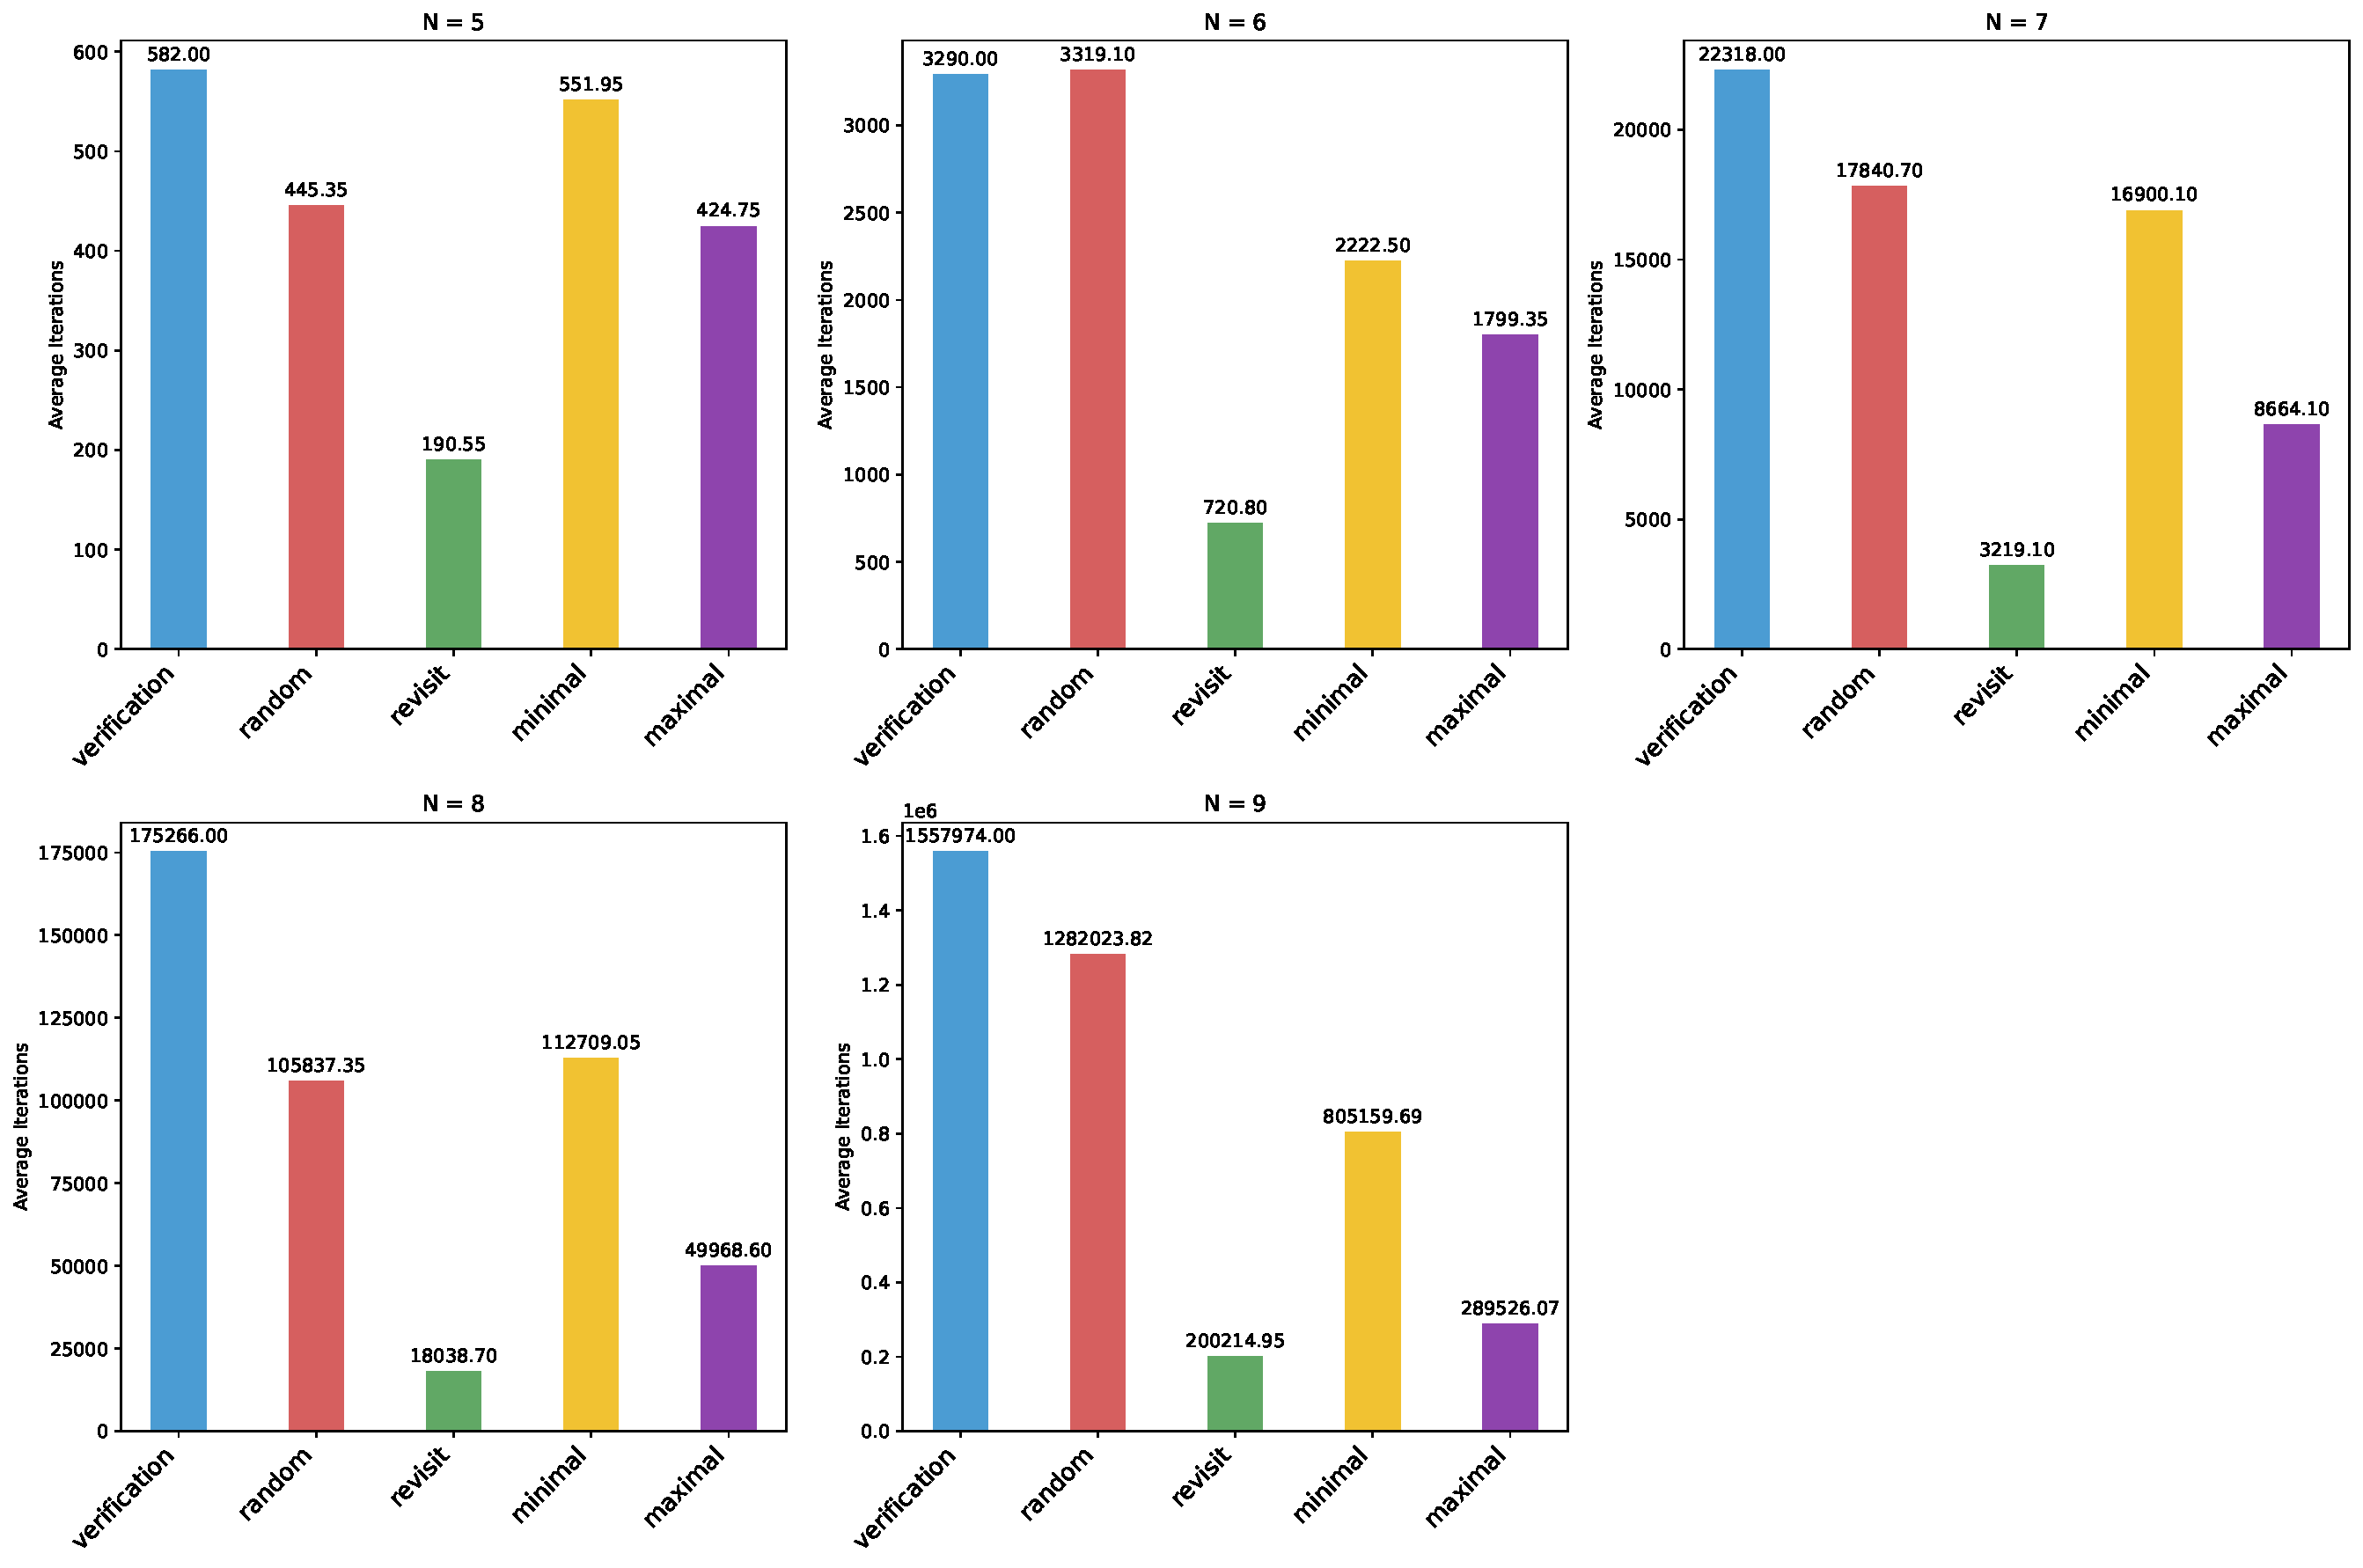
\includegraphics[scale=0.3]{figure/long-assert/fuzz_iter.pdf}
	\caption{Average iterations to detect the bug (varying assertion)}
	\label{long-assert-N-iter}
\end{figure}


\begin{figure}[h!tbp]
	\centering
	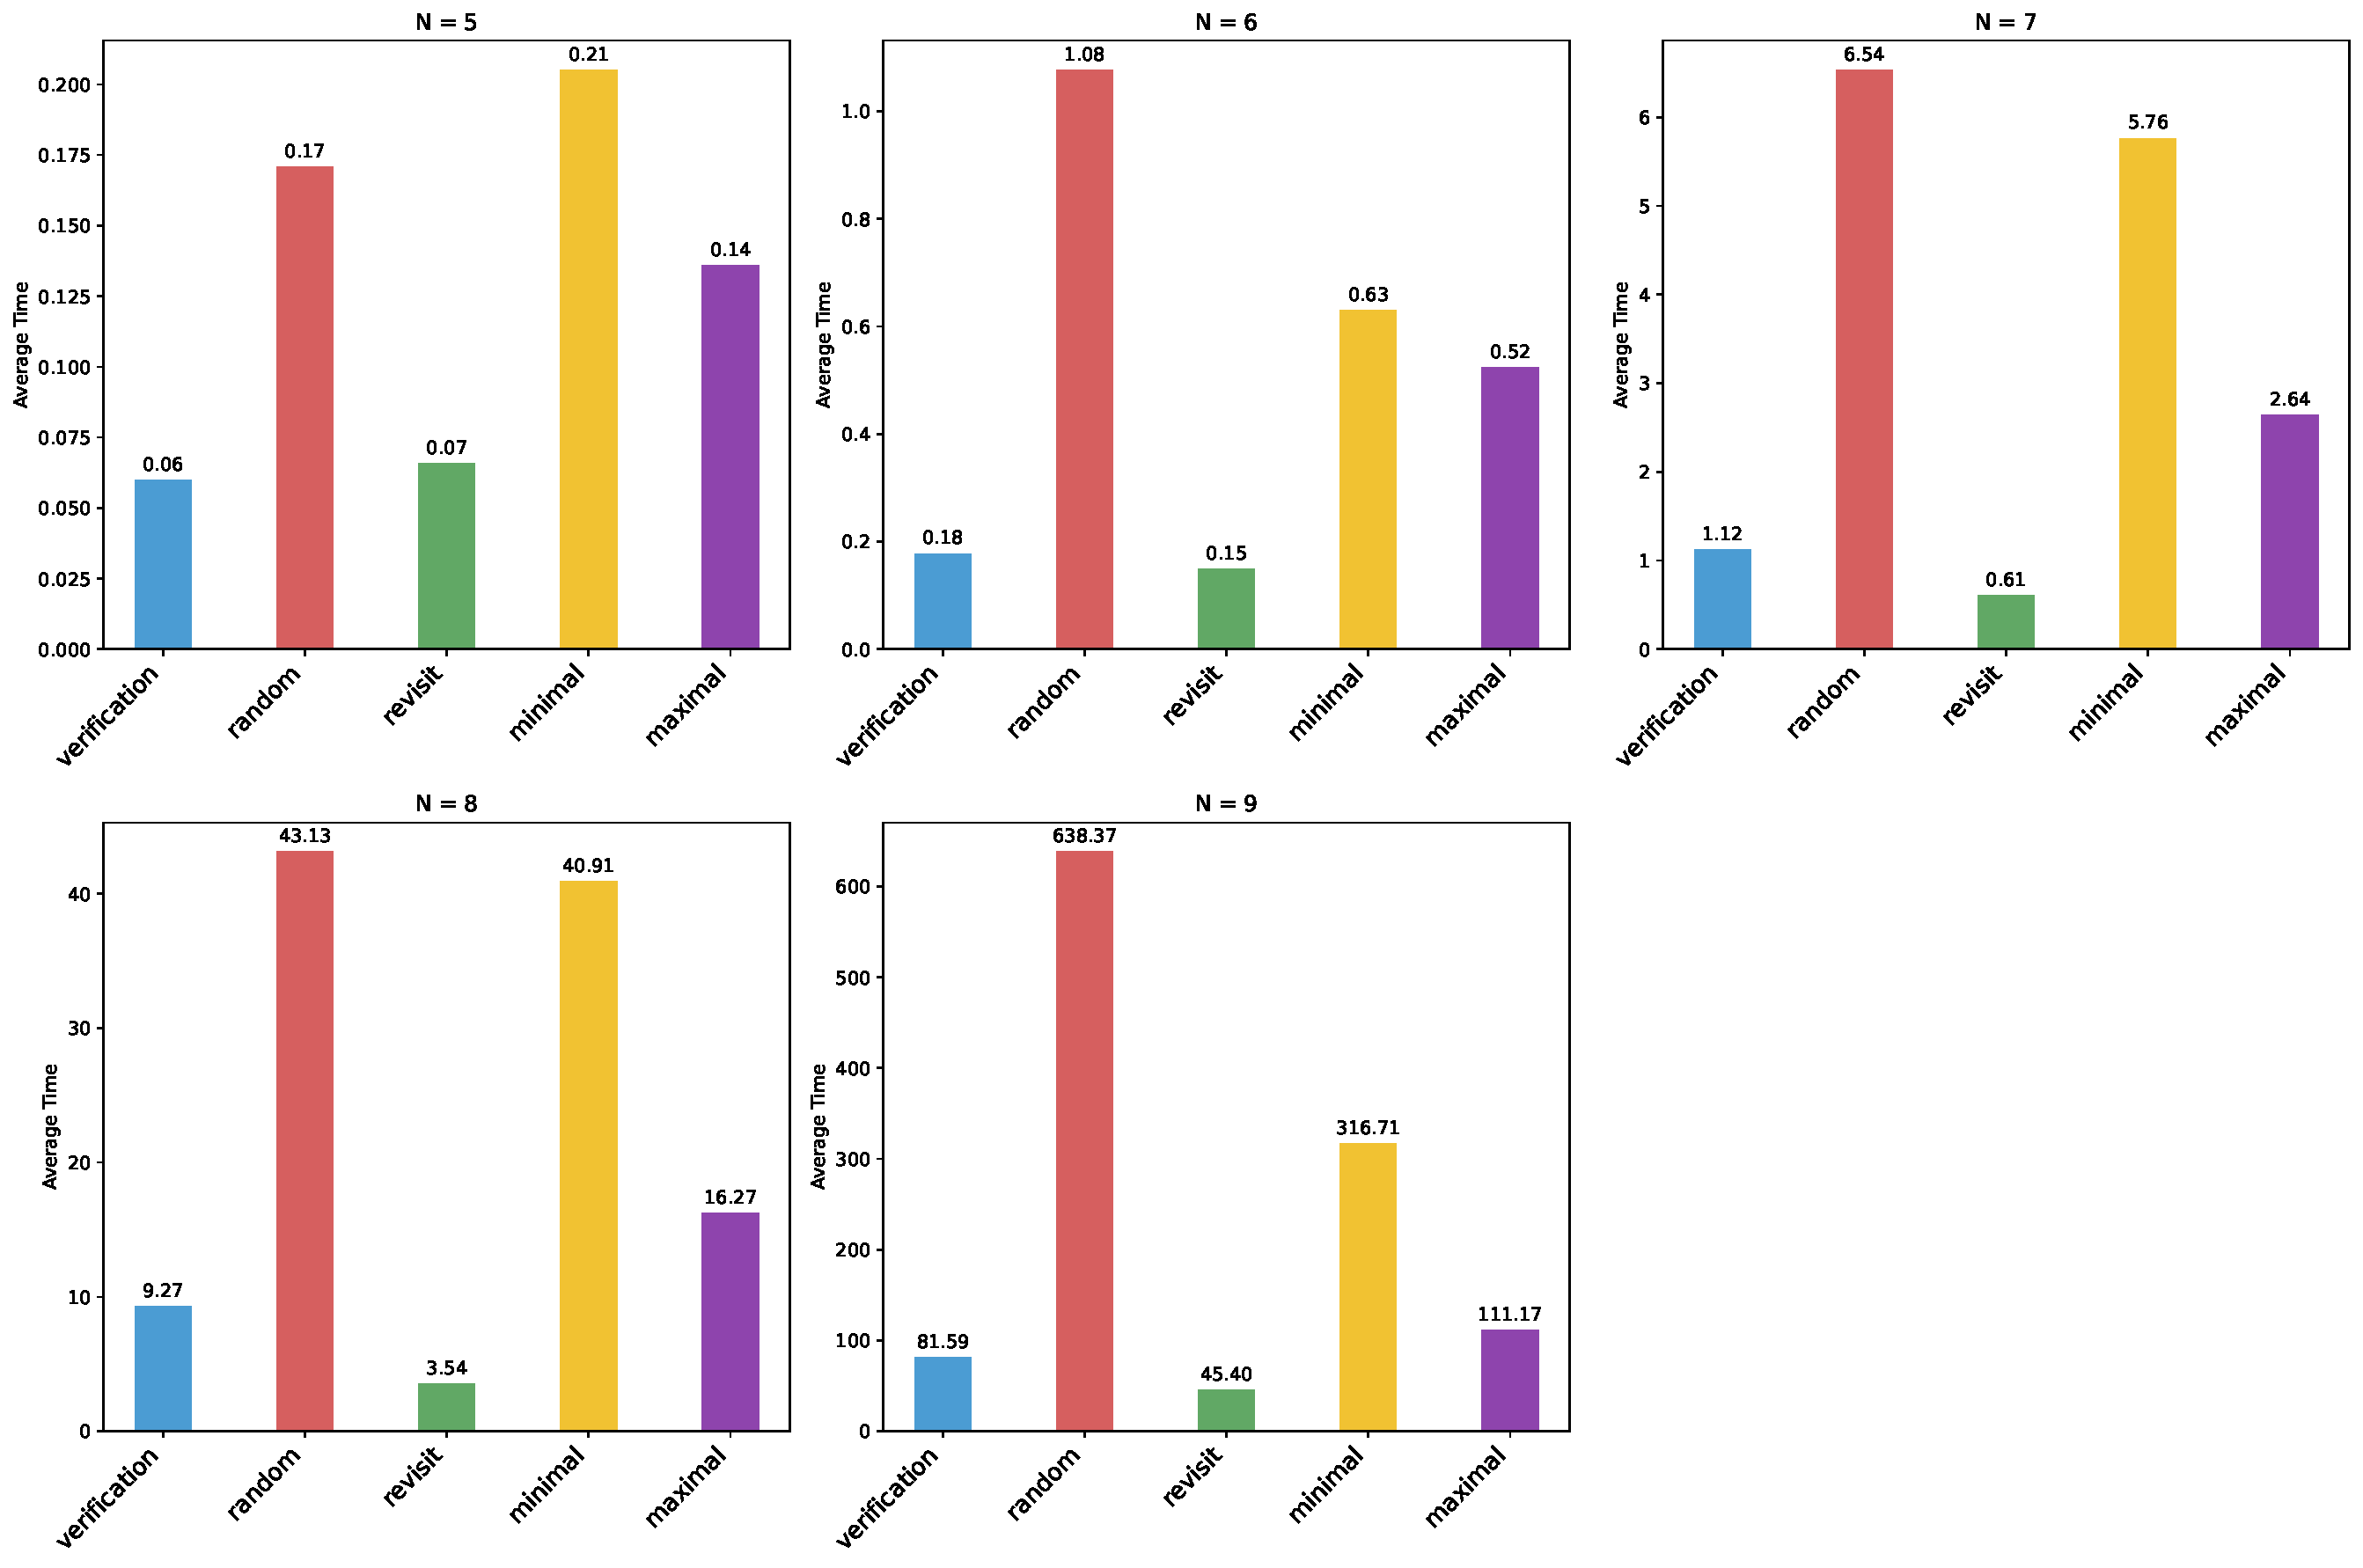
\includegraphics[scale=0.3]{figure/long-assert/fuzz_time.pdf}
	\caption{Average time to detect the bug (varying assertion)}
	\label{long-assert-N-time}
\end{figure}